\documentclass[11pt]{article}
\usepackage[review]{acl}
\usepackage{times}
\usepackage{latexsym}
\usepackage[T1]{fontenc}
\usepackage[utf8]{inputenc}
\usepackage{microtype}
%\usepackage{inconsolata} % not installed here; only affects typewriter font
\usepackage{graphicx}
\usepackage{amsmath}
\usepackage{booktabs}
\usepackage{tabularx}
\usepackage{xltabular}
\usepackage{array}
\usepackage{textcomp}
\usepackage{placeins}
\usepackage{enumitem}

\renewcommand{\topfraction}{0.9}\renewcommand{\bottomfraction}{0.8}\renewcommand{\textfraction}{0.07}
\renewcommand{\floatpagefraction}{0.8}\renewcommand{\dbltopfraction}{0.9}\renewcommand{\dblfloatpagefraction}{0.8}
\newcommand{\nohdpunct}{}
\newcommand{\appendixsection}[1]{\section{#1}}
\newenvironment{acknowledgments}{\section*{Acknowledgments}}{}

\title{Same Sentences, Different Order: Arrangement, Noun Familiarity\\and What Small Transformers Carry Forward}

\author{Anonymous submission}

\begin{document}
\maketitle

\begin{abstract}
Training pipelines decide how text is arranged, but arrangement is rarely tested with content held fixed. We trained small transformers on artificial languages in which the same sentences about 32 kinds of object came in different orders, then described one object of a new kind and measured how much more the models expected the next object of that kind to keep its shape than its colour. We tested with three kinds of noun: tokens never seen in training, the same tokens given an embedding typical of trained nouns, and nouns from training. For all three, grouping sentences by kind raised this expectation relative to random order, only when kinds had a fixed feature, and more when nearby sentences described different objects than when they described the same object again. How much of the context's shape the models carried forward depended on the noun: strongly for unseen tokens, little for typical-looking ones, and not at all for trained nouns whose kind always had one shape. When a kind's shape changed from pass to pass, trained nouns carried it forward, but only after the same noun. Models trained on one short fixed file memorised it, and their effects differed in size. Probes built on unseen tokens therefore measure arrangement and the representation of the test noun together.
\end{abstract}

\section{Introduction}
Every training pipeline arranges its text. It packs documents into windows, orders them and, more and more, generates synthetic text whose layout someone chooses \citep{shi2024,zhao2024}. Work on training data mostly asks about content \citep{warstadt2023,feng2024}. Arrangement alone, with content held fixed, is rarely tested, although natural text differs in it: a word that has appeared once in a document is far more likely to appear again soon than its frequency predicts \citep{church2000}, and talk to toddlers returns to the same objects in clusters \citep{slone2023}. In transformers, burstiness of this kind decides whether in-context learning emerges \citep{chan2022}. We ask a smaller question: with the same sentences, what does arrangement teach a model to expect about the next mention of a kind?

We need a regularity that holds across items, so that arrangement can make it easier or harder to see. We borrow one from word learning: things with the same name tend to share a shape \citep{landau1988,kemp2007}. We give a model one sentence about an object of a new kind, \emph{A snerg is a krannish pulek skorli thing}, where the three adjectives name a shape, a colour and a texture, and ask how much more it expects a second snerg to keep the shape than the colour. We use this only as a probe of what transformers learn from their data; our claims are about transformers, not children.

Such probes usually use a nonce noun the model has never seen, so that nothing it has stored about the noun can answer for it. But a never-seen token has an untrained embedding, and what a model does with it may reflect that embedding rather than what it learned from the arrangement. In a study of mutual exclusivity in child-scale models, apparent effects with nonce tokens reflected embedding similarity \citep{cacioli2026me}. We therefore test with three kinds of noun: unseen tokens, the same tokens given an embedding typical of trained nouns, and nouns from training.

We trained 510 small transformers (3.4M to 25.6M parameters) on artificial languages whose content and order we control, with every pass of a corpus arranged afresh. Two corpora act as controls: in one nothing is fixed within a kind (a negative control for grouping), and in the other each kind's shape changes from pass to pass, so that only the context can say which shape comes next (a positive control for using the context with the noun). We find:
\begin{enumerate}[leftmargin=*,itemsep=1pt,topsep=2pt]
\item \textbf{The direction of the arrangement effects held for every noun.} Grouping sentences by kind raised the expectation that shape persists relative to colour, only when kinds had a fixed feature, and more when nearby sentences described different objects rather than the same object again.
\item \textbf{The size depended on the noun.} The models carried the context's shape forward strongly for unseen tokens, little for typical-looking tokens and not at all for trained nouns. An apparent effect of moderate clustering held only for unseen tokens.
\item \textbf{The positive control worked.} When a kind's shape changed between passes, trained nouns carried it forward, but only after the same noun.
\item \textbf{Fixed files changed the result.} Models trained on one fixed file, each position read 160 to 290 times, memorised it, and their effects differed in size.
\end{enumerate}
The confirmatory tests were registered in stages; some registrations were written after earlier results were known, and the comparison across kinds of noun was added afterwards and is exploratory (Appendix~\ref{app:A}).

\section{Related work}
\textbf{Arrangement and order.} Packing related documents into one window improves how pretrained models use their context \citep{shi2024,zhao2024}. Curricula that order examples by difficulty have given mixed results \citep{bengio2009,rohde1999,diehlmartinez2023}. At child scale, the local order of child-directed speech affected what models learned, while its global order by age did not \citep{feng2024}. We hold content fixed and vary only local arrangement.

\textbf{In-context and in-weights learning.} \citet{chan2022} found that in-context learning emerged when items of a class appeared in bursts, more strongly when item meanings were dynamic rather than fixed, and traded off against learning stored in the weights; \citet{singh2023} showed that it can fade as the stored solution takes over, and \citet{reddy2024} traced its onset to induction heads. Our test nouns span the same trade-off, from tokens with nothing stored to nouns with a stored feature.

\textbf{Artificial languages, nonce words and repeated data.} Artificial languages let a model's preferences be traced to its input \citep{mccoy2020,white2021,kallini2024}, and nonce words are the usual way to test generalisation to a new item \citep{thrush2020}. Such studies typically reuse one generated corpus over many passes, from about two to a few dozen in these examples \citep{mccoy2020,kallini2024,murty2023}. The number of passes matters: training long on fixed data changed hierarchical generalisation \citep{murty2023}; at a fixed budget, small sets of repeated examples beat larger sets of single-use examples on synthetic maths tasks \citep{charton2024}; and the BabyLM Challenge capped training at ten epochs in 2025, judging tens or hundreds of repeated exposures developmentally implausible \citep{charpentier2025}.

\textbf{Shape bias in networks.} Networks trained on images or artificial objects can show a shape bias \citep{ritter2017,feinman2018}, and a hierarchical Bayesian model learns it from how kinds vary \citep{kemp2007}. We use it as a probe, not as a target.

\section{Method}
\label{sec:method}
\subsection{Corpora and arrangements}
Each corpus describes 32 kinds of object, each named by a novel noun (\emph{wug}, \emph{dax}, \ldots), with 14 exemplars per kind. Each exemplar has a shape, a colour and a texture, each a novel word from a list of ten, and is described by one sentence in one of five frames (Figure~\ref{fig:1}; Appendix~\ref{app:I}). Shape is named in all five frames, colour in three and texture in one. The frames are the same in every corpus, so every conclusion rests on comparisons between corpora. The 448 sentences of a corpus (1,664 for Objects), each used once, make up one pass. Table~\ref{tab:terms} defines the corpora, arrangements and measures.

\begin{table}[t]
\centering
\small
\setlength{\tabcolsep}{3pt}
\begin{tabular}{@{}p{0.27\columnwidth}p{0.69\columnwidth}@{}}
\toprule
Term & Meaning \\
\midrule
Regular & Each kind keeps one shape; colour and texture vary. \\
No stable feature & Shape drawn at random per exemplar; nothing fixed within a kind (negative control). \\
Objects & 13 objects per kind, each described four times. \\
Reassigned & Each kind gets a new shape in every pass and keeps it within that pass (positive control). \\
\midrule
Random order & Every pass shuffled. \\
Grouped order & Sentences about a kind cut into runs of four; runs shuffled across kinds. \\
Same- / different-object run & Four descriptions of one object / of four objects of one kind. \\
\midrule
Fresh / fixed text & Every pass arranged anew, no window read twice / one fixed file, each position read 160 to 290 times. \\
$\Delta$ & Preference (nats) for a continuation that repeats a feature of the context sentence. \\
Index & $\Delta_{\text{shape}} - \Delta_{\text{colour}}$. \\
\bottomrule
\end{tabular}
\caption{Terms used in this paper.}
\label{tab:terms}
\end{table}

\textbf{Arrangement.} In random order every pass is shuffled. In grouped order the sentences about each kind are cut into runs of four and the runs are shuffled across kinds; every sentence occurs as often as in random order. A graded order keeps each run with a set probability and otherwise splits it; the one used here gives clustering of 3.5 on a statistic, $B$, that is 0.9 for random order and 23 for grouped order (Appendix~\ref{app:I}).

\textbf{Fresh and fixed text.} Our main models were trained on fresh text: 7,500 passes of a corpus (2,100 for Objects), each arranged with its own random draw, 34 to 35 million tokens in all, read in non-overlapping 128-token windows so that no window was read twice. For comparison, other models were trained on one fixed file of 11,648 sentences (about 120,000 tokens) with windows at random positions, so that each position was read 160 to 290 times (Table~\ref{tab:1}, Appendix~\ref{app:I}).

\begin{figure*}[t]
\centering
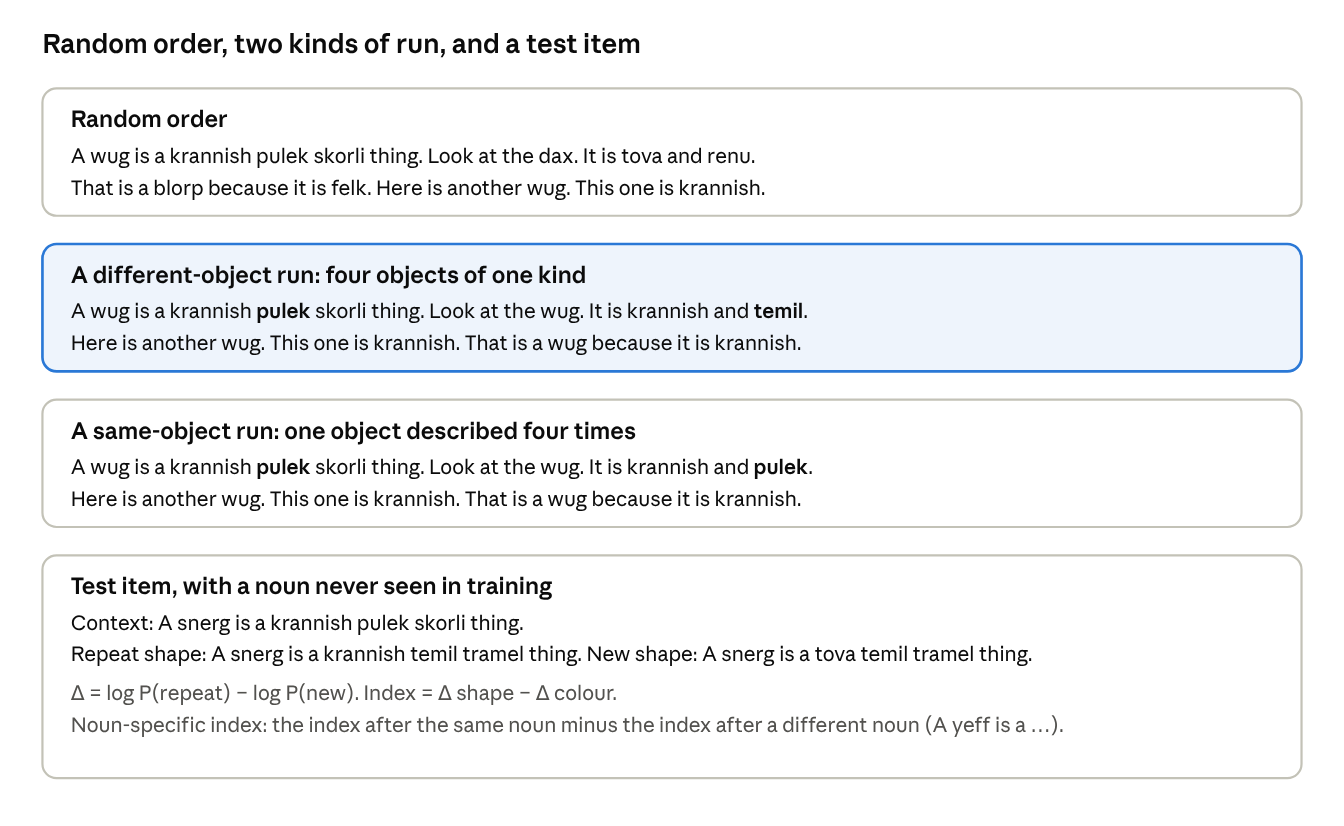
\includegraphics[width=0.78\textwidth]{figures/figure1.png}
\caption{Random order, the two kinds of run, and a test item. In the different-object run the colour changes from one wug to the next; in the same-object run it repeats.}
\label{fig:1}
\end{figure*}

\subsection{Models and test}\label{sec:test}
We trained decoder-only transformers of 3.4, 11.0 and 25.6 million parameters (4 to 8 layers) for 5,000 to 10,000 steps, with five seeds per condition at each size; a seed sets the corpus, the weights and the batch order (Appendix~\ref{app:C}). Every artificial word is one token.

Each test item gives the model one frame-1 sentence about an exemplar, then two continuations that differ in one word: one repeats the probed feature and one does not (Figure~\ref{fig:1}). $\Delta$ is the difference in summed log probability between them. Trained models generally prefer words they have just seen, so we report the index, $\Delta_{\text{shape}} - \Delta_{\text{colour}}$, which cancels copying that affects both features equally, together with $\Delta$ for each feature. Measured on the changed word alone, every result is nearly the same (Appendix~\ref{app:L}). With one exemplar, nothing in the context shows which feature is fixed, so differences between conditions come from training.

\textbf{Three kinds of test noun.} \emph{Unseen tokens} are eight nouns that never occur in training; their input embeddings were never trained, because a tie between input and output embeddings was lost on the training hardware. \emph{Typical tokens} are the same eight nouns with their input embedding replaced by the mean embedding of the 32 trained nouns plus a distinct offset of typical length, so that they look like ordinary nouns but remain distinct from each other (exploratory; Appendix~\ref{app:L}). \emph{Trained nouns} occur in training; to keep items comparable, an item never offers a trained noun its own kind's fixed feature, so in Regular corpora both continuations give it a shape it never had (Appendix~\ref{app:F}). Each item is also given with a different noun in the continuations; the \textbf{noun-specific index} is the index after the same noun minus the index after a different noun.

\textbf{Statistics.} Models of three sizes with the same seed share a corpus, so the five seeds are the units of replication. We average sizes within each seed and compare conditions by paired $t$ tests over the five seed means (4 degrees of freedom); estimates and 95\% intervals are these seed-level values. Registered contrasts were one-sided with \citet{holm1979} correction within each registration and concern unseen tokens; results given with a Holm $p$ were registered, and all others, including every result for typical tokens and trained nouns in Regular corpora, are exploratory. Every contrast reported as reliable had the same direction at all three model sizes.

\section{Results}\label{sec:results}

\begin{table*}[t]
\centering
\small
\setlength{\tabcolsep}{4.5pt}
\begin{tabular}{@{}llrrrrrr@{}}
\toprule
 & & \multicolumn{3}{c}{Index (shape over colour)} & \multicolumn{3}{c}{$\Delta$ shape} \\
\cmidrule(lr){3-5}\cmidrule(l){6-8}
Corpus & Order ($B$) & Unseen & Typical & Trained & Unseen & Typical & Trained \\
\midrule
Regular & Random (0.9) & \textminus{}1.56 & \textminus{}1.54 & \textminus{}0.02 & \textminus{}1.55 & \textminus{}1.52 & 0.03 \\
Regular & Graded (3.5) & 1.28 & \textminus{}1.41 & \textminus{}0.13 & 1.18 & \textminus{}1.52 & 0.06 \\
Regular & Grouped (23) & 9.52 & 1.46 & 2.00 & 6.88 & \textminus{}0.72 & 0.06 \\
No stable feature & Grouped (23) & \textminus{}3.98 & \textminus{}3.51 & \textminus{}3.75 & \textminus{}3.88 & \textminus{}3.51 & \textminus{}3.58 \\
Objects & Same-object runs (24) & 5.87 & \textminus{}1.85 & \textminus{}0.55 & 6.87 & \textminus{}1.17 & \textminus{}0.09 \\
Objects & Different-object runs (24) & 7.60 & \textminus{}1.25 & 0.03 & 8.05 & \textminus{}1.14 & 0.04 \\
Reassigned & Random (0.9) & 0.21 & 0.18 & 0.14 & 0.22 & 0.24 & 0.24 \\
Reassigned & Grouped (23) & 9.80 & 3.87 & 11.65 & 6.81 & 1.17 & 10.01 \\
\bottomrule
\end{tabular}
\caption{Models trained on fresh text, one exemplar, same noun in the continuation (nats; mean of 15 models per row, five seeds). Unseen: nouns never seen in training (untrained embeddings). Typical: the same nouns with an embedding typical of trained nouns. Trained: nouns from training, never offered their own kind's shape. Appendix~\ref{app:E} gives standard deviations, model sizes and every fixed-file condition; Appendix~\ref{app:L} gives colour and texture.}
\label{tab:2}
\end{table*}

\subsection{The direction of the arrangement effects held for every noun}\label{sec:persist}
With unseen tokens, Regular models trained in random order came to expect the shape to \emph{change}, at \textminus{}1.56 nats [\textminus{}2.45,~\textminus{}0.67], and the same sentences in grouped order gave 9.52 (Table~\ref{tab:2}). Three registered contrasts held, in the same direction and in all five seeds, for every kind of test noun (Table~\ref{tab:contrasts}). Grouping raised the index relative to random order. The gain needed a fixed feature: with nothing fixed within kinds, grouped models expected the shape to change, for every noun (\textminus{}3.51 to \textminus{}3.98). And runs that described different objects gave a larger index than runs describing one object four times, because after same-object runs the models expected colour to repeat as well, as it does in those runs ($\Delta$ colour 0.99 against 0.46 with unseen tokens). Fixed-file models, the only ones trained with colour fixed instead of shape, show that the preference follows the fixed feature: grouped Colour stable models favoured colour, at \textminus{}3.20 (Holm $p<.001$; Appendix~\ref{app:E}).

\begin{table}[t]
\centering
\small
\setlength{\tabcolsep}{2.5pt}
\begin{tabular}{@{}p{0.31\columnwidth}ccc@{}}
\toprule
Contrast & Unseen & Typical & Trained \\
\midrule
Grouped $-$ random & 11.08 & 3.00 & 2.03 \\
 & {\scriptsize[9.57, 12.59]} & {\scriptsize[1.79, 4.21]} & {\scriptsize[1.68, 2.37]} \\
Regular $-$ No stable, grouped & 13.50 & 4.98 & 5.76 \\
 & {\scriptsize[11.48, 15.52]} & {\scriptsize[3.42, 6.53]} & {\scriptsize[4.98, 6.53]} \\
Different $-$ same object & 1.72 & 0.60 & 0.58 \\
 & {\scriptsize[0.54, 2.90]} & {\scriptsize[0.26, 0.93]} & {\scriptsize[0.30, 0.86]} \\
$B = 3.5$ $-$ random & 2.84 & 0.13 & \textminus{}0.10 \\
 & {\scriptsize[1.41, 4.27]} & {\scriptsize[\textminus{}0.34, 0.59]} & {\scriptsize[\textminus{}0.34, 0.14]} \\
\bottomrule
\end{tabular}
\caption{Seed-level differences in the index (nats, 95\% intervals over five seeds). For unseen tokens these are registered tests (Holm $p$ = $<$.001, $<$.001, .008 and .005); the other columns are exploratory. The first three were positive in all five seeds for every noun.}
\label{tab:contrasts}
\end{table}

One registered result did not generalise. Clustering at $B = 3.5$, near that of object labels in speech to children, raised the index with unseen tokens (2.84 [1.41,~4.27], Holm $p=.005$), but not with typical tokens or trained nouns. We therefore make no claim about moderate clustering.

These expectations follow the corpora. In grouped order the next sentence is about the same kind 72\% of the time and then always repeats the shape; in random order it is about the same kind 3\% of the time. A learner that predicts each feature from the previous sentence alone, ignoring the noun, gives a reference index that the unseen-token results tracked across conditions (Pearson $r = .88$ over eight conditions; exploratory and descriptive; Appendix~\ref{app:E}). The reference predicts the direction of the same- against different-object contrast, so that contrast is what the corpora warrant. It does not predict the expectation of change, which is near zero in the reference for random order and for No stable feature corpora. That expectation persisted with typical tokens in random order (\textminus{}1.54) and with every noun in No stable feature corpora, but not with trained nouns in random order (\textminus{}0.02). We have no tested account of it.

\subsection{How much shape is carried depends on the noun}\label{sec:noun}
The noun decided how much of the context's shape the models carried forward (Table~\ref{tab:2}, right). In grouped Regular corpora, $\Delta$ shape was 6.88 [5.22,~8.54] with unseen tokens, \textminus{}0.72 with typical tokens and 0.06 [\textminus{}0.27,~0.39] with trained nouns; the Objects corpora showed the same pattern. With typical tokens and trained nouns, what remained of the grouping effect came mostly from colour: grouped models expected colour to change ($\Delta$ colour \textminus{}2.18 and \textminus{}1.94; Appendix~\ref{app:L}). For trained nouns, whose items never offer the noun's own shape, $\Delta$ shape near zero means that a shape given in the context was not carried to the next mention. This is consistent with the models predicting a trained kind's shape from its noun, but our items cannot test that.

So the large shape effects seen with unseen tokens are not a general property of what grouping teaches. They are what grouping teaches a model about a noun it cannot place. This parallels the trade-off between in-context and in-weights learning \citep{chan2022,singh2023}: the less a model can tell from the noun, the more it takes from the context.

\subsection{Positive control: a shape the noun cannot predict}
Reassigned corpora keep the run structure but remove any stored shape: a kind's shape changes from pass to pass, so only the previous sentence about the kind shows which shape comes next. Trained on them in grouped order, models tested with trained nouns carried the shape forward after the same noun ($\Delta$ shape 10.01) and not after a different one (0.08). Their noun-specific index was 11.24 [10.44,~12.03] (Holm $p<.001$), close to the 11.4 that the corpus warrants. The noun-specific index was smaller with unseen tokens (0.37 [0.24,~0.49], Holm $p=.001$) and with typical tokens (0.70 [0.31,~1.10], exploratory), which the models cannot recognise as a known kind. In random order, Reassigned corpora taught neither a preference for shape nor a dependence on the noun, for any noun (index 0.14 to 0.21). So the test detects a noun-tied use of the context when the data require it, and trained nouns took up the context's shape exactly where their noun could not predict it.

\subsection{Fixed files memorise and change the result}
Fixed-file models memorised their files: their loss was 0.08 to 0.11 nats per token on their own file but 0.66 to 1.26 on a new arrangement of the same sentences, while fresh-text models scored 0.28 to 0.55 on both (Appendix~\ref{app:C}). The effects changed with it. With unseen tokens, the grouping effect was about half the size (6.02 [5.24,~6.79] against 11.08), and in random order the index was 0.47, not reliably above zero (Holm $p=.061$), rather than \textminus{}1.56; early in training, while their loss was near that of fresh-text models, these models also gave \textminus{}0.4 to \textminus{}1.5 (exploratory). Every contrast measured in both regimes had the same direction, but not the same size. Our fixed files were read 160 to 290 times, more than most artificial-language studies use, although BabyLM entries have trained for hundreds to thousands of epochs \citep{warstadt2023}, and fixed against fresh text changes both the number of passes and the variety of windows. The result adds to evidence that repeated passes over fixed data change what is learned \citep{murty2023,charton2024}.

\begin{table}[t]
\centering
\small
\setlength{\tabcolsep}{3pt}
\begin{tabular}{@{}p{0.47\columnwidth}lr@{}}
\toprule
Registered test & Estimate [95\% CI] & Holm $p$ \\
\midrule
\multicolumn{3}{@{}l}{\emph{Supported}}\\
Grouped above random order & 11.08 [9.57, 12.59] & $<$.001 \\
$B = 3.5$ above random order & 2.84 [1.41, 4.27] & .005 \\
Grouped: Regular above No stable & 13.50 [11.48, 15.52] & $<$.001 \\
Grouped: Colour stable below No stable$^{\dagger\circ}$ & 2.76 [1.99, 3.52] & $<$.001 \\
Index rises with $\log B$ (slope)$^{\dagger\circ}$ & 1.63 [1.46, 1.80] & $<$.001 \\
Different-object above same-object runs & 1.72 [0.54, 2.90] & .008 \\
Noun-specific, Reassigned, trained nouns & 11.24 [10.44, 12.03] & $<$.001 \\
Noun-specific, Reassigned, unseen tokens & 0.37 [0.24, 0.49] & .001 \\
\quad above grouped Regular & 0.25 [0.10, 0.39] & .005 \\
Speech to children above written text, $B$ & 2.14 [1.55, 2.91] & $<$.001 \\
Pythia index rises with size & $\rho = .92$ & .003 \\
\multicolumn{3}{@{}l}{\emph{Not supported}}\\
Random-order index above zero$^{\dagger\circ}$ & 0.47 & .061 \\
512-token window raises index$^{\dagger\circ}$ & 0.03 [\textminus{}0.44, 0.50] & .87 \\
\quad at $B = 3.6$ (reversed)$^{\dagger\circ}$ & \textminus{}0.63 [\textminus{}0.90, \textminus{}0.37] & 1.00 \\
Noun-specific, random order, unseen$^{\dagger\circ}$ & 0.005 & .46 \\
Pythia noun-specific index rises with size$^{\circ}$ & $\rho = $ \textminus{}.42 & 1.00 \\
Pythia noun-specific index above zero$^{\circ}$ & \textminus{}0.15 & 1.00 \\
Pythia index rises over training & $\rho = $ \textminus{}.34 & 1.00 \\
BabyLM baselines above zero & 0.47; 0.37 & .52; .12 \\
\bottomrule
\end{tabular}
\caption{Main registered tests, all with unseen test tokens. Estimates are seed-level differences, or the index itself where no contrast is named; fresh text unless marked $^{\dagger}$ (fixed files). $^{\circ}$: registered after related results were known; the others were registered before the related models were trained or scored, or before the transcripts were read. Holm $p$ is the test named in the registration, corrected within it: the seed-level test for fresh text, a mixed model or Welch test for fixed files, and for pretrained models the tests in Appendix~\ref{app:K}. Before a loader error was corrected, two fixed-file verdicts differed (Appendix~\ref{app:A}). Units are nats except for $B$ and $\rho$. Appendix~\ref{app:A} gives all 32 registered hypotheses.}
\label{tab:main}
\end{table}

\section{Discussion}
Arranging the same sentences differently changed what small transformers expected of the next mention of a kind, and the direction of that change held whether the test noun was unseen, typical-looking or trained. Grouping helped only when kinds had a fixed feature, and runs of different objects taught the fixed feature more selectively than the same object described again, as the corpora warrant. How much the models took from the context depended on the noun. They carried the context's shape forward for nouns they could not place, and for trained nouns only where the noun could not predict the shape, and then only after the same noun. We identify the conditions that produce these behaviours, not their mechanism; carrying a word forward is the kind of behaviour attributed to induction heads \citep{olsson2022}, but we did not examine attention. People show related patterns: blocked study helps learners find what members of a category share \citep{carvalho2014}, and varied exemplars taught toddlers more than near-identical ones \citep{perry2010}. We note the parallel without taking our results as evidence about how children learn.

Two methodological points follow. First, probes built on unseen tokens measure arrangement and the representation of the test noun together. Here a registered effect of moderate clustering, and most of the size of every effect, depended on the test noun being unlike any trained noun; in a study of mutual exclusivity, nonce-token effects likewise reflected embedding similarity \citep{cacioli2026me}. Studies that use nonce words should vary how they are represented. Second, small-scale experiments on data should report how many passes they make over fixed text; arranging each pass afresh removes memorisation at no cost in content.

We also measured the same clustering statistic in natural corpora: object labels were more clustered in speech to young children than in adult conversation or written text, though nearly half of the nearby repetitions in speech to children returned to the same object (Appendix~\ref{app:J}). Pythia models gained a shape-over-colour expectation with size, but none preferred shape over texture, and evidence that they tied it to the noun was weak (Appendix~\ref{app:K}). These are descriptive comparisons, not tests.

\section*{Limitations}
The artificial language has 32 kinds, three dimensions and five frames that name shape more often than colour or texture; conclusions rest on comparisons between corpora that share the frames. The models are small (3.4M to 25.6M parameters), trained with one recipe and five seeds per condition, and we do not know how the effects scale. Unseen tokens had untrained input embeddings because an intended tie between input and output embeddings was lost; typical tokens are one choice of a familiar-looking embedding, and the comparison across kinds of noun was made after the registrations. Trained-noun items never offer the noun's own shape, so they show that the context's shape was not carried forward, not how the stored shape is used. The expectation that shape changes, in random order and in No stable feature corpora, is unexplained. Colour stable corpora, half of the levels of clustering and several controls exist only as fixed files, which their models memorised; fixed and fresh text differ in both the number of passes and the variety of windows. The registrations were made in stages, several after earlier results were known, and a loader error, corrected before the final analyses, had changed two verdicts. All corpora are English.

\section*{Ethics statement}
The corpus analysis in Appendix~\ref{app:J} is a secondary analysis of archived, de-identified transcripts (CHILDES, CABank) used under their terms; no data were collected from people, and no transcript excerpts are reproduced. Code, corpora, results and all trained models will be released; anonymised copies are provided as supplementary material.

\section*{Use of AI assistants}
An AI assistant (Claude, Anthropic) was used to help design analyses, write code, draft and edit text and check citations, and as the second coder in a consistency check of the corpus coding. The authors are responsible for all content, including the accuracy of every citation.

\bibliography{refs}

\appendix
\onecolumn
\appendixsection{Registration record}\label{app:A}
\setcounter{table}{0}\renewcommand{\thetable}{A\arabic{table}}
\setcounter{figure}{0}\renewcommand{\thefigure}{A\arabic{figure}}
In the appendices and the registrations, Study 1 is the training experiments (Section~\ref{sec:background} and Appendices~\ref{app:A} to~\ref{app:I}), Study 2 the natural corpora (Appendix~\ref{app:J}) and Study 3 the pretrained models (Appendix~\ref{app:K}).

All registrations are in one public project on the Open Science Framework (link withheld for review; an anonymised view-only link is in the supplementary material), and each states what was known when it was written. Table A1 lists them, Table A2 gives the label each registration uses for each row of Table A4, and Table A4 gives every registered hypothesis and its result.

\begin{table}[!htbp]
\caption{Registrations. Each was written before the models it concerns were trained or scored, or before the transcripts were read.}
\label{tab:5}
\small
\begin{tabularx}{\textwidth}{>{\hsize=0.903\hsize\raggedright\arraybackslash}X>{\hsize=0.602\hsize\raggedright\arraybackslash}X>{\hsize=1.247\hsize\raggedright\arraybackslash}X>{\hsize=1.247\hsize\raggedright\arraybackslash}X}
\toprule
Registration & Written & Rows of Table A4 & Known when it was written \\
\midrule
Original & 2 Mar 2026 & Corpora, models and controls (Appendix D) & Nothing trained \\
Amendment 1 & 7 Oct 2026 & 1, 2, 3, 6, 16 & Random-order models trained and scored on an earlier test, with the old loader; no grouped model trained \\
Amendment 2 & 7 Oct 2026 & 7 (texture added as a co-primary test) & No grouped model trained \\
Amendment 3 & 8 Oct 2026 & 23, 24, 25 & Study 1 results for rows 1 to 3, 6, 7 and 16 (old loader); no pretrained model scored \\
Amendment 4 & 8 Oct 2026 & 20, 21 & Studies 1 and 3 results; no transcript read \\
Amendment 5 & 9 Oct 2026 & 4, 5, 8, 9, 17, 18, 19, 22 & All earlier results (Study 1 with the old loader); four reviews of a draft; five exploratory checks, including the confound of the noun with another \\
Amendment 6 & 11 Oct 2026 & 11, 12, 13 & Amendment 5 results (old loader); a prediction for the new models fitted to them \\
Amendment 7 & 12 Oct 2026 & 10, 14, 15 & All results, with corrected scores \\
Amendment 8 & 15 Oct 2026 & 26 to 32 & All results, with corrected scores; three rounds of reviews, which noted that fixed-file models memorised their files and that the novel-noun test was uninformative; no fresh-text model trained \\
Amendment 9 & 23 Oct 2026 & Familiarity study (Appendix~\ref{app:M}) & All results above; no familiarity corpus built \\
Amendment 10 & 24 Oct 2026 & Recurrence, frames, rows and pretrained models (Appendix~\ref{app:N}) & Amendment 9 results and a blind review of them; no Amendment 10 corpus used, model trained or pretrained model run on its items \\
\bottomrule
\end{tabularx}
\end{table}

\begin{table}[!htbp]
\caption{Rows of Table A4 and the labels used in the registrations.}
\label{tab:6}
\footnotesize\setlength{\tabcolsep}{3.5pt}
\begin{tabularx}{\textwidth}{>{\hsize=0.747\hsize\raggedright\arraybackslash}X>{\hsize=1.493\hsize\raggedright\arraybackslash}X>{\hsize=0.747\hsize\raggedright\arraybackslash}X>{\hsize=1.173\hsize\raggedright\arraybackslash}X>{\hsize=0.747\hsize\raggedright\arraybackslash}X>{\hsize=1.173\hsize\raggedright\arraybackslash}X>{\hsize=0.747\hsize\raggedright\arraybackslash}X>{\hsize=1.173\hsize\raggedright\arraybackslash}X}
\toprule
Row & Label & Row & Label & Row & Label & Row & Label \\
\midrule
1 & H4b & 9 & H13b & 17 & H14a & 25 & H8 \\
2 & H1b & 10 & H22 & 18 & H14b & 26 & H23 \\
3 & H2b & 11 & H17 & 19 & H15 & 27 & H24 \\
4 & H11 & 12 & H18 & 20 & H9 & 28 & H25 \\
5 & H12 & 13 & H19 & 21 & H10 & 29 & H26 \\
6 & H5b colour & 14 & H20 & 22 & H16 & 30 & H27 \\
7 & H5b texture & 15 & H21 & 23 & H6 & 31 & H28 \\
8 & H13a & 16 & H3b & 24 & H7 & 32 & H29 \\
\bottomrule
\end{tabularx}
\end{table}

\textbf{The loading correction.} The model code ties the input embedding to the output layer. On the graphics card used for training (through DirectML) the tie was lost, so every Study 1 model was trained and saved with two separate matrices. The first version of the scoring code rebuilt each model with the tie in place before loading its weights, so the output matrix overwrote the input embedding. We found this on 12 October 2026, fixed the loader, and rescored all 315 Study 1 models then trained, 461 intermediate checkpoints of the random and grouped Regular models and the trained-noun items, with the same items. A check on eight randomly chosen models confirmed the fix: mean loss on each model's own training corpus was 0.07 to 0.16 nats per token with the corrected loader, close to the last logged training loss (0.08 to 0.23; dropout is off at test), and 0.58 to 1.97 with the old one. Studies 2 and 3 were not affected. The old scores are kept in the repository.

\begin{table}[!htbp]
\caption{Study 1 registered tests before and after the correction (shape-over-colour index, nats). Rows 10, 14 and 15 were registered and scored after the correction.}
\label{tab:7}
\small
\begin{tabularx}{\textwidth}{>{\hsize=0.373\hsize\raggedright\arraybackslash}X>{\hsize=1.067\hsize\raggedright\arraybackslash}X>{\hsize=1.013\hsize\raggedright\arraybackslash}X>{\hsize=1.547\hsize\raggedright\arraybackslash}X}
\toprule
Row & Old loader & Corrected & Verdict before $\rightarrow$ after \\
\midrule
1 & 1.36 vs 0.18 & 6.49 vs 0.47 & Supported $\rightarrow$ supported \\
2 & 0.18 & 0.47 & Not supported $\rightarrow$ not supported \\
3 & 0.18 vs 0.09 & 0.47 vs \textminus{}0.25 & Not supported $\rightarrow$ supported \\
4 & difference 1.45 & difference 6.93 & Supported $\rightarrow$ supported \\
5 & difference 1.17 & difference 2.76 & Supported $\rightarrow$ supported \\
6 & 1.36 vs 0.80 & 6.49 vs 2.12 & Supported $\rightarrow$ supported \\
7 & 1.10 vs \textminus{}0.04 & 5.36 vs 0.46 & Supported $\rightarrow$ supported \\
8 & slope 0.29 & slope 1.63 & Supported $\rightarrow$ supported \\
9 & 0.24 vs 0.18 & 1.43 vs 0.47 & Not supported $\rightarrow$ supported \\
11 & 0.21 vs 0.18 & 0.50 vs 0.47 & Not supported $\rightarrow$ not supported \\
12 & 0.29 vs 0.24 & 0.80 vs 1.43 & Not supported $\rightarrow$ not supported (reversed) \\
13 & 0.21 vs \textminus{}0.08 & 0.50 vs 0.10 & Supported $\rightarrow$ supported \\
16 & difference 0.0007 & difference 0.005 & Equivalent to zero $\rightarrow$ equivalent to zero \\
\bottomrule
\end{tabularx}
\end{table}

\FloatBarrier\clearpage
{\footnotesize\setlength{\tabcolsep}{3.5pt}
\begin{xltabular}{\textwidth}{>{\hsize=0.200\hsize\raggedright\arraybackslash}X>{\hsize=1.933\hsize\raggedright\arraybackslash}X>{\hsize=1.267\hsize\raggedright\arraybackslash}X>{\hsize=1.133\hsize\raggedright\arraybackslash}X>{\hsize=0.667\hsize\raggedright\arraybackslash}X>{\hsize=0.800\hsize\raggedright\arraybackslash}X>{\hsize=1.000\hsize\raggedright\arraybackslash}X}
\multicolumn{7}{@{}p{\linewidth}@{}}{\refstepcounter{table}\label{tab:8}{\normalsize\textbf{Table \thetable}\newline All registered hypotheses and results; registered secondary analyses are reported in the text. Rows 1 to 16 concern fixed-file models and rows 26 to 32 fresh-text models. Seed-level tests average the three sizes within each of five seeds (t-based 95\% intervals, two-sided; tests one-sided unless marked, 4 degrees of freedom), so a one-sided test can be below .05 while the two-sided interval includes zero (row 13). The registered p is the test named in the registration, one-sided unless marked, Holm-corrected within its registration; for rows 26 to 32 it is the seed-level test, corrected within rows 26 to 29 and within rows 30 to 32. Corpus intervals resample sources and then documents; Pythia and BabyLM intervals resample nouns.}}\\[6pt]
\toprule
\# & Prediction & Result (nats) & Seed-level difference [95\% CI] & Seed-level p & Registered p & Verdict \\
\midrule
\endfirsthead
\toprule \# & Prediction & Result (nats) & Seed-level difference [95\% CI] & Seed-level p & Registered p & Verdict \\ \midrule \endhead
\bottomrule \endlastfoot
 & 1. Does grouping teach the fixed feature? &  &  &  &  &  \\
1 & Grouped order gives a higher index than random order & 6.49 vs 0.47 & 6.02 [5.24,~6.79] & $<$~.001 & $<$~.001 & Supported \\
2 & Random order gives an index above zero & 0.47 & 0.47 [\textminus{}0.61,~1.56] & .15 & .061 & Not supported \\
3 & Random order: Regular above Mixed-slot & 0.47 vs \textminus{}0.25 & 0.73 [\textminus{}0.69,~2.15] & .11 & .032 & Supported by the registered test, not at the seed level \\
4 & Grouped: Regular above No stable feature & 6.49 vs \textminus{}0.44 & 6.93 [5.47,~8.40] & $<$~.001 & $<$~.001 & Supported \\
5 & Grouped: Colour stable below No stable feature & \textminus{}3.20 vs \textminus{}0.44 & 2.76 [1.99,~3.52] & $<$~.001 & $<$~.001 & Supported \\
6 & Grouped: Regular above Mixed-slot, shape over colour & 6.49 vs 2.12 & 4.37 [1.98,~6.76] & .004 & $<$~.001 & Supported \\
7 & Grouped: Regular above Mixed-slot, shape over texture & 5.36 vs 0.46 & 4.89 [2.69,~7.10] & .002 & $<$~.001 & Supported \\
8 & The index rises with log B across six orders & Slope 1.63 (SE 0.10) & 1.63 [1.46,~1.80] & $<$~.001 & $<$~.001 & Supported \\
9 & B = 3.6 above random order & 1.43 vs 0.47 & 0.96 [0.63,~1.28] & $<$~.001 & $<$~.001 & Supported \\
10 & The same, Objects corpora, different-object runs & 1.18 vs 0.22 & 0.96 [0.37,~1.54] & .005 & $<$~.001 & Supported \\
26 & Fresh text: grouped order gives a higher index than random order & 9.52 vs \textminus{}1.56 & 11.08 [9.57,~12.59] & $<$~.001 & $<$~.001 & Supported \\
27 & Fresh text: B = 3.5 above random order & 1.28 vs \textminus{}1.56 & 2.84 [1.41,~4.27] & .003 & .005 & Supported \\
28 & Fresh text, grouped: Regular above No stable feature & 9.52 vs \textminus{}3.98 & 13.50 [11.48,~15.52] & $<$~.001 & $<$~.001 & Supported \\
 & 2. What kind of grouping helps? &  &  &  &  &  \\
11 & 512-token window above 128, random order & 0.50 vs 0.47 & 0.03 [\textminus{}0.44,~0.50] & .44 & .87 & Not supported \\
12 & 512-token window above 128, B = 3.6 & 0.80 vs 1.43 & \textminus{}0.63 [\textminus{}0.90,~\textminus{}0.37] & .003 (two-sided) & 1.00 & Not supported; reliably reversed \\
13 & 512-token window: Regular above No stable feature & 0.50 vs 0.10 & 0.40 [\textminus{}0.04,~0.85] & .032 & .045 & Supported; weak \\
14 & Grouped: different-object above same-object runs & 5.65 vs 2.99 & 2.66 [1.57,~3.75] & .001 & $<$~.001 & Supported \\
15 & B = 3.6: different-object above same-object runs & 1.18 vs 0.45 & 0.73 [0.15,~1.32] & .013 & $<$~.001 & Supported \\
29 & Fresh text, grouped: different-object above same-object runs & 7.60 vs 5.87 & 1.72 [0.54,~2.90] & .008 & .008 & Supported \\
 & 3. Is the expectation tied to the noun? &  &  &  &  &  \\
16 & Fixed files, random order: index higher after the same noun (novel nouns) & Difference 0.005; equivalent to zero (p = .001), but the novel nouns were untrained (Section~\ref{sec:background}) &  &  & .46 & Not supported \\
30 & Shape reassigned, grouped: noun-specific index above zero, novel nouns & 0.37 & 0.37 [0.24,~0.49] & $<$~.001 & .001 & Supported \\
31 & The same, above grouped Regular (fresh text) & 0.37 vs 0.12 & 0.25 [0.10,~0.39] & .005 & .005 & Supported \\
32 & Shape reassigned, grouped: noun-specific index above zero, nouns from training & 11.24 & 11.24 [10.44,~12.03] & $<$~.001 & $<$~.001 & Supported \\
17 & Pythia: noun-specific index rises with size (wording matched) & $\rho$ = \textminus{}.42 &  &  & 1.00 & Not supported \\
18 & Pythia 410M to 12B: noun-specific index above zero (wording matched) & \textminus{}0.15 (SE 0.12) &  &  & 1.00 & Not supported \\
19 & Pythia: 410M above 160M across ten training seeds & 0.15 vs \textminus{}0.15 &  &  & .012 & Supported \\
 & 4. What do natural input and pretrained models show? &  &  &  &  &  \\
20 & Speech to children: B above 1 & 3.57 [3.13,~4.30] &  &  & $<$~.001 & Supported \\
21 & Speech to children above written text & 3.57 vs 1.43; difference 2.14 [1.55,~2.91] &  &  & $<$~.001 & Supported \\
22 & Speech to children differs from adult conversation (two-sided) & 3.57 vs 2.33; difference 1.24 [0.51,~2.03] &  &  & $<$~.001 & Supported; higher \\
23 & Pythia: index rises with size & $\rho$ = .92 &  &  & .003 & Supported \\
24 & Pythia: index rises over training & Mean within-size $\rho$ = \textminus{}.34 &  &  & 1.00 & Not supported \\
25 & BabyLM baselines (10M, 100M words): index above zero & 0.47 [\textminus{}1.05,~1.93]; 0.37 [\textminus{}0.04,~0.73] &  &  & .52; .12 & Not supported \\
\end{xltabular}}

\textbf{Fresh text and shape reassignment.} Rows 26 to 32 were registered on 15 October 2026, after reviews of the manuscript had noted that fixed-file models memorised their files and that the test with novel nouns was uninformative, and before any fresh-text model was trained. The corpora were built, and their checksums registered, before training. Amendment 8 names the conditions by their folder names (for example reassigned\_grouped).

\FloatBarrier
\appendixsection{Deviations from the registrations}\label{app:B}
\setcounter{table}{0}\renewcommand{\thetable}{B\arabic{table}}
\setcounter{figure}{0}\renewcommand{\thefigure}{B\arabic{figure}}
\begin{enumerate}
\item Two registered analyses are not reported here: the Bayesian reference model of Amendment 1, which is in the repository, and the prediction of Amendment 6 for the 512-token models, which had been fitted to scores later corrected (Appendix A).
\item Added after registration: the seed-level tests for rows 1 to 3 and 6 to 8, the seed-level intervals, and intervals for the differences between natural corpora (from the registered two-stage bootstrap). Effective clustering was computed before it was registered as the scale for Figure~\ref{fig:2} and is reported as exploratory (Table~\ref{tab:3}).
\item The two models of about 70 billion parameters were scored with Apple's MLX library, because PyTorch crashed the machine; on smaller models the two differed by 0.003 to 0.010 nats on average.
\item In the hand coding of Study 2, a rule for labels not used for a physical object was added during coding and applied by both coders, and one pair of the reliability subset was discussed with an AI assistant and left out of the agreement check.
\end{enumerate}

Smaller technical changes (software versions, download addresses, a stale file in one public model repository) are listed in the repository.

\FloatBarrier
\appendixsection{Model and training settings}\label{app:C}
\setcounter{table}{0}\renewcommand{\thetable}{C\arabic{table}}
\setcounter{figure}{0}\renewcommand{\thefigure}{C\arabic{figure}}
\begin{table}[!htbp]
\caption{AdamW (betas 0.9 and 0.95, weight decay 0.1), linear warm-up then cosine decay, dropout 0.1, untied input and output embeddings. Fixed-file models read windows starting at random positions in the corpus; fresh-text models read non-overlapping windows, each at most once, in random order (the 3.4M and 25.6M models used about 60\% of the windows available, the 11.0M models 94 to 96\%). Byte-pair tokeniser with 351 entries for the Regular corpora and 314 to 339 for the other corpus families; every artificial word is one token. Seeds 42, 123, 456, 789 and 1001 each set the corpus, the initial weights and the batch order. Checkpoints were saved every 500 steps. Training ran on one Windows PC through DirectML.}
\label{tab:8x1}
\small
\begin{tabularx}{\textwidth}{>{\hsize=1.750\hsize\raggedright\arraybackslash}X>{\hsize=0.750\hsize\raggedright\arraybackslash}X>{\hsize=0.750\hsize\raggedright\arraybackslash}X>{\hsize=0.750\hsize\raggedright\arraybackslash}X}
\toprule
Setting & 3.4M & 11.0M & 25.6M \\
\midrule
Layers, heads, width & 4, 4, 256 & 6, 8, 384 & 8, 8, 512 \\
Feed-forward width & 1,024 & 1,536 & 2,048 \\
Steps & 5,000 & 8,000 & 10,000 \\
Batch (128-token windows) & 32 & 32 & 16 \\
Batch (512-token windows) & 8 & 8 & 4 \\
Peak learning rate & 3 $\times$ $10^{-4}$ & 2 $\times$ $10^{-4}$ & 1 $\times$ $10^{-4}$ \\
Warm-up steps & 200 & 400 & 500 \\
\bottomrule
\end{tabularx}
\end{table}

\begin{table}[!htbp]
\caption{Memorisation. Mean next-token loss (nats per token) on 300 windows from each model's own training text and from a new arrangement of the same sentences (100 further passes, 27 for the Objects corpora, never used in training); 15 models per cell. At the seed level, the gap between the two losses was larger for fixed-file than for fresh-text models by 0.57 to 1.16 nats, with every interval excluding zero.}
\label{tab:9}
\footnotesize
\begin{tabularx}{\textwidth}{>{\hsize=1.629\hsize\raggedright\arraybackslash}X>{\hsize=0.618\hsize\raggedright\arraybackslash}X>{\hsize=1.067\hsize\raggedright\arraybackslash}X>{\hsize=0.618\hsize\raggedright\arraybackslash}X>{\hsize=1.067\hsize\raggedright\arraybackslash}X}
\toprule
Corpus & Fixed file: own file & Fixed file: new arrangement & Fresh text: own text & Fresh text: new arrangement \\
\midrule
Regular, random & 0.11 & 1.25 & 0.55 & 0.55 \\
Regular, B 3.6 (fresh: 3.5) & 0.10 & 1.26 & 0.54 & 0.54 \\
Regular, grouped & 0.09 & 0.85 & 0.35 & 0.35 \\
No stable feature, grouped & 0.09 & 1.00 & 0.39 & 0.39 \\
Objects, same-object runs, grouped & 0.08 & 0.66 & 0.28 & 0.28 \\
Objects, different-object runs, grouped & 0.09 & 0.76 & 0.32 & 0.32 \\
\bottomrule
\end{tabularx}
\end{table}

\FloatBarrier
\appendixsection{Further content controls}\label{app:D}
\setcounter{table}{0}\renewcommand{\thetable}{D\arabic{table}}
\setcounter{figure}{0}\renewcommand{\thefigure}{D\arabic{figure}}
Six further corpora, each trained in random order only, change one thing about Regular. \textbf{No kind label}: the nouns are removed, with no other marker of the kind. \textbf{Paraphrased}: the nouns are removed and replaced by randomly chosen category markers. \textbf{Weak label}: nouns appear in 25\% of sentences and category markers in the rest. \textbf{Frequency matched}: the same feature words as often as in Regular, with the fixed feature of each kind drawn at random from shape, texture or none. \textbf{Added noise}: Regular with 7\% of exemplars given a wrong fixed feature. \textbf{Feature swap}: 16 kinds keep their shape and 16 keep their texture.

\begin{table}[!htbp]
\caption{Further controls, random order, 15 models each. In random order every index is small, so these corpora say little about what grouping would do with them.}
\label{tab:10}
\small
\begin{tabularx}{\textwidth}{>{\hsize=1.385\hsize\raggedright\arraybackslash}X>{\hsize=0.769\hsize\raggedright\arraybackslash}X>{\hsize=0.667\hsize\raggedright\arraybackslash}X>{\hsize=1.179\hsize\raggedright\arraybackslash}X}
\toprule
Corpus & Shape over colour, mean (SD) & Shape over texture & Noun-specific index \\
\midrule
Regular (for comparison) & 0.47 (0.90) & 0.51 & 0.005 \\
No kind label & 0.06 (0.49) & 0.44 & \textminus{}0.004 \\
Paraphrased & 0.41 (0.44) & 0.60 & \textminus{}0.025 \\
Weak label & 0.09 (0.50) & \textminus{}0.52 & 0.008 \\
Frequency matched & \textminus{}0.22 (0.63) & \textminus{}0.40 & \textminus{}0.033 \\
Added noise & \textminus{}0.43 (0.67) & 0.44 & \textminus{}0.038 \\
Feature swap & 0.69 (0.77) & 0.60 & \textminus{}0.017 \\
\bottomrule
\end{tabularx}
\end{table}

\FloatBarrier
\clearpage
\appendixsection{Robustness}\label{app:E}
\setcounter{table}{0}\renewcommand{\thetable}{E\arabic{table}}
\setcounter{figure}{0}\renewcommand{\thefigure}{E\arabic{figure}}
\FloatBarrier
{\small
\begin{xltabular}{\textwidth}{>{\hsize=0.467\hsize\raggedright\arraybackslash}X>{\hsize=1.267\hsize\raggedright\arraybackslash}X>{\hsize=1.267\hsize\raggedright\arraybackslash}X}
\multicolumn{3}{@{}p{\linewidth}@{}}{\refstepcounter{table}\label{tab:11}{\normalsize\textbf{Table \thetable}\newline p values for the Study 1 rows of Table A4 under paired tests at the seed level and over the 15 matched models (one-sided unless marked).}}\\[6pt]
\toprule
Row & Seed level (5 seeds) & Matched models (15) \\
\midrule
\endfirsthead
\toprule Row & Seed level (5 seeds) & Matched models (15) \\ \midrule \endhead
\bottomrule \endlastfoot
1 & $<$~.001 & $<$~.001 \\
2 & .15 & .031 \\
3 & .11 & .014 \\
4 & $<$~.001 & $<$~.001 \\
5 & $<$~.001 & $<$~.001 \\
6 & .004 & $<$~.001 \\
7 & .002 & $<$~.001 \\
8 & $<$~.001 &  \\
9 & $<$~.001 & $<$~.001 \\
10 & .005 & $<$~.001 \\
11 & .44 & .44 \\
12 & .003 (two-sided) & .003 (two-sided) \\
13 & .032 & .015 \\
14 & .001 & $<$~.001 \\
15 & .013 & $<$~.001 \\
26 & $<$~.001 & $<$~.001 \\
27 & .003 & $<$~.001 \\
28 & $<$~.001 & $<$~.001 \\
29 & .008 & $<$~.001 \\
30 & $<$~.001 & $<$~.001 \\
31 & .005 & .010 \\
32 & $<$~.001 & $<$~.001 \\
\end{xltabular}}

\FloatBarrier\clearpage
{\footnotesize\setlength{\tabcolsep}{3.5pt}
\begin{xltabular}{\textwidth}{>{\hsize=1.851\hsize\raggedright\arraybackslash}X>{\hsize=0.574\hsize\raggedright\arraybackslash}X>{\hsize=0.702\hsize\raggedright\arraybackslash}X>{\hsize=0.702\hsize\raggedright\arraybackslash}X>{\hsize=1.085\hsize\raggedright\arraybackslash}X>{\hsize=1.085\hsize\raggedright\arraybackslash}X}
\multicolumn{6}{@{}p{\linewidth}@{}}{\refstepcounter{table}\label{tab:11x1}{\normalsize\textbf{Table \thetable}\newline Shape-over-colour index by model size (one exemplar), and with two or four exemplars in the context that share their shape (all sizes). Rows marked fresh are fresh-text models; the rest are fixed-file models. In grouped Regular models, two or four exemplars lowered the index: a run of a kind has four sentences, so a fifth sentence about the same kind is rare (Section~\ref{sec:background}). In grouped No stable feature and Colour stable models, where shape varies within a kind, more exemplars sharing a shape lowered the index ($\Delta$ shape \textminus{}0.64, \textminus{}1.93 and \textminus{}3.42 with one, two and four exemplars in grouped No stable feature models), for which we have no tested account; in random-order Regular models, too, the index was lower with two or four exemplars than with one.}}\\[6pt]
\toprule
Condition & 3.4M & 11.0M & 25.6M & Two exemplars & Four exemplars \\
\midrule
\endfirsthead
\toprule Condition & 3.4M & 11.0M & 25.6M & Two exemplars & Four exemplars \\ \midrule \endhead
\bottomrule \endlastfoot
Regular, random, fresh & \textminus{}1.00 & \textminus{}0.87 & \textminus{}2.81 & \textminus{}1.83 & \textminus{}2.19 \\
Regular, B 3.5, fresh & 1.37 & 2.27 & 0.21 & 2.05 & \textminus{}0.53 \\
Regular, grouped, fresh & 7.43 & 12.57 & 8.56 & 7.88 & 4.24 \\
No stable feature, grouped, fresh & \textminus{}1.21 & \textminus{}4.80 & \textminus{}5.92 & \textminus{}5.41 & \textminus{}7.24 \\
Objects, same-object, grouped, fresh & 8.21 & 4.60 & 4.81 & 3.86 & 0.62 \\
Objects, different-object, grouped, fresh & 9.96 & 6.29 & 6.54 & 5.78 & 2.13 \\
Reassigned, random, fresh & \textminus{}0.06 & 0.33 & 0.35 & 0.59 & 0.23 \\
Reassigned, grouped, fresh & 6.52 & 14.05 & 8.85 & 9.62 & 8.26 \\
Regular, random & 0.33 & 0.71 & 0.38 & \textminus{}0.64 & \textminus{}0.10 \\
Regular, B 1.4 & 0.73 & 1.05 & 0.70 & \textminus{}0.01 & 0.32 \\
Regular, B 3.6 & 0.97 & 2.05 & 1.27 & 0.60 & 1.06 \\
Regular, B 7 & 1.85 & 2.89 & 1.45 & 1.23 & 1.15 \\
Regular, B 12 & 3.18 & 4.53 & 2.88 & 2.85 & 2.43 \\
Regular, grouped & 6.41 & 6.83 & 6.23 & 5.24 & 4.30 \\
Mixed-slot, random & \textminus{}0.11 & \textminus{}0.45 & \textminus{}0.21 & 0.29 & 0.29 \\
Mixed-slot, grouped & 2.24 & 2.35 & 1.76 & 2.60 & 2.04 \\
No stable feature, random & \textminus{}0.10 & \textminus{}0.33 & \textminus{}0.12 & \textminus{}0.17 & \textminus{}0.44 \\
No stable feature, grouped & \textminus{}0.41 & \textminus{}0.28 & \textminus{}0.63 & \textminus{}1.77 & \textminus{}3.26 \\
Colour stable, random & \textminus{}0.04 & \textminus{}0.70 & \textminus{}0.51 & \textminus{}0.76 & \textminus{}0.76 \\
Colour stable, grouped & \textminus{}2.11 & \textminus{}3.72 & \textminus{}3.77 & \textminus{}4.50 & \textminus{}5.34 \\
Regular, random, 512 & 0.30 & 0.51 & 0.70 & 0.51 & 0.32 \\
Regular, B 3.6, 512 & 0.31 & 1.02 & 1.06 & 0.93 & 0.82 \\
No stable feature, random, 512 & 0.21 & 0.04 & 0.05 & \textminus{}0.10 & \textminus{}0.23 \\
Objects, random & 0.36 & 0.44 & \textminus{}0.13 & 0.38 & 1.02 \\
Objects, same-object, B 3.6 & 0.22 & 0.98 & 0.14 & 0.32 & 1.22 \\
Objects, different-object, B 3.6 & 0.83 & 1.75 & 0.96 & 1.49 & 2.18 \\
Objects, same-object, grouped & 3.00 & 3.33 & 2.62 & 1.30 & 1.34 \\
Objects, different-object, grouped & 6.18 & 5.43 & 5.34 & 4.54 & 4.14 \\
\end{xltabular}}

\textbf{Noun-specific index.} At the seed level, the noun-specific index was equivalent to zero (two one-sided tests, $\pm$0.2 nats) in 25 of the 26 fixed-file conditions; the exception was same-object runs at B = 3.6 (\textminus{}0.11, p = .058). No condition exceeded 0.15 nats in absolute value. These nulls are uninformative, because the models did not track novel nouns (Section~\ref{sec:background}). As a further check, for the 60 models in the random and grouped Regular and grouped Objects conditions we compared the log probability of the same novel noun after the context and the word A with the mean over the other seven novel nouns. The difference was no more than 0.032 nats in absolute value in every model, and positive on about half the items. Because the novel nouns were never training targets, this check also depends on output weights that training only pushed down, so it is weaker evidence than the trained-noun contrast in Section 3.5.

\textbf{Correction across all tests.} Holm correction was applied within each registered family of tests, as registered. Every row of Table A4 with a Holm-adjusted p below .001 has an unadjusted p below .001, and so stays below .05 under Holm correction across all 32 tests.

\textbf{What the corpora reward.} For every pair of consecutive sentences in each training corpus (five seeds pooled), Table E3 gives the share about the same kind and how often the second sentence repeats the first one's shape or colour. The noun-blind reference index is D(shape) \textminus{} D(colour), where D = ln p \textminus{} ln((1 \textminus{} p)/9) and p is the share of pairs that repeat that feature, with ten values per dimension; it is what a learner that predicts each feature from the previous sentence alone would show on a one-exemplar item. The noun-aware reference computes the same index separately for pairs about the same kind and pairs about different kinds (add-0.5 smoothing).

\begin{table}[!htbp]
\caption{What each training corpus says about the next sentence, and the models' shape-over-colour index for comparison. Rows marked fresh describe fresh text, counted on 100 held-out passes arranged by the same rule (27 for the Objects corpora); the rest describe the fixed files. All values in nats except the shares. Code is in the repository.}
\label{tab:11x2}
\scriptsize\setlength{\tabcolsep}{3.5pt}
\begin{tabularx}{\textwidth}{>{\hsize=3.073\hsize\raggedright\arraybackslash}X>{\hsize=0.878\hsize\raggedright\arraybackslash}X>{\hsize=0.732\hsize\raggedright\arraybackslash}X>{\hsize=0.732\hsize\raggedright\arraybackslash}X>{\hsize=0.732\hsize\raggedright\arraybackslash}X>{\hsize=0.805\hsize\raggedright\arraybackslash}X>{\hsize=0.732\hsize\raggedright\arraybackslash}X>{\hsize=0.732\hsize\raggedright\arraybackslash}X>{\hsize=0.585\hsize\raggedright\arraybackslash}X}
\toprule
Corpus & Next sentence same kind & Shape repeats, same kind & Shape repeats, other kind & Colour repeats, same kind & Noun-blind reference & Noun-aware, same kind & Noun-aware, other kind & Model index \\
\midrule
Regular, random, fresh & 0.03 & 1.00 & 0.07 & 0.10 & \textminus{}0.01 & 11.7 & \textminus{}0.35 & \textminus{}1.56 \\
Regular, B 3.5, fresh & 0.11 & 1.00 & 0.07 & 0.09 & 0.65 & 13.1 & \textminus{}0.37 & 1.28 \\
Regular, grouped, fresh & 0.72 & 1.00 & 0.07 & 0.10 & 3.25 & 14.9 & \textminus{}0.38 & 9.52 \\
No stable feature, grouped, fresh & 0.72 & 0.10 & 0.10 & 0.10 & 0.02 & 0.0 & \textminus{}0.01 & \textminus{}3.98 \\
Objects, same-object, grouped, fresh & 0.76 & 1.00 & 0.07 & 0.99 & 0.39 & 8.4 & \textminus{}0.35 & 5.87 \\
Objects, different-object, grouped, fresh & 0.76 & 1.00 & 0.07 & 0.10 & 3.43 & 14.9 & \textminus{}0.29 & 7.60 \\
Reassigned, random, fresh & 0.03 & 1.00 & 0.10 & 0.10 & 0.27 & 8.2 & 0.01 & 0.21 \\
Reassigned, grouped, fresh & 0.72 & 1.00 & 0.10 & 0.10 & 3.30 & 11.4 & \textminus{}0.02 & 9.80 \\
Regular, random & 0.03 & 1.00 & 0.07 & 0.10 & \textminus{}0.01 & 10.3 & \textminus{}0.35 & 0.47 \\
Regular, B 1.4 & 0.04 & 1.00 & 0.07 & 0.10 & 0.13 & 10.8 & \textminus{}0.35 & 0.83 \\
Regular, B 3.6 & 0.11 & 1.00 & 0.07 & 0.10 & 0.70 & 11.7 & \textminus{}0.31 & 1.43 \\
Regular, B 7 & 0.22 & 1.00 & 0.07 & 0.10 & 1.23 & 12.4 & \textminus{}0.37 & 2.06 \\
Regular, B 12 & 0.38 & 1.00 & 0.07 & 0.09 & 1.91 & 13.0 & \textminus{}0.40 & 3.53 \\
Regular, grouped & 0.72 & 1.00 & 0.07 & 0.10 & 3.25 & 13.5 & \textminus{}0.33 & 6.49 \\
No stable feature, grouped & 0.72 & 0.10 & 0.10 & 0.10 & 0.03 & 0.0 & 0.06 & \textminus{}0.44 \\
Colour stable, grouped & 0.72 & 0.10 & 0.10 & 1.00 & \textminus{}3.26 & \textminus{}12.5 & 0.38 & \textminus{}3.20 \\
Objects, same-object, B 3.6 & 0.11 & 1.00 & 0.07 & 0.70 & 0.19 & 8.6 & \textminus{}0.35 & 0.45 \\
Objects, different-object, B 3.6 & 0.11 & 1.00 & 0.07 & 0.11 & 0.74 & 11.6 & \textminus{}0.25 & 1.18 \\
Objects, same-object, grouped & 0.76 & 1.00 & 0.07 & 0.99 & 0.37 & 7.0 & \textminus{}0.39 & 2.99 \\
Objects, different-object, grouped & 0.76 & 1.00 & 0.07 & 0.10 & 3.39 & 13.5 & \textminus{}0.41 & 5.65 \\
\bottomrule
\end{tabularx}
\end{table}

\begin{table}[!htbp]
\caption{Study 1 results for models trained on fixed files, in nats after one exemplar with the same noun; 15 models per row, 128-token windows unless marked.}
\label{tab:12}
\footnotesize\setlength{\tabcolsep}{3.5pt}
\begin{tabularx}{\textwidth}{>{\hsize=1.384\hsize\raggedright\arraybackslash}X>{\hsize=2.116\hsize\raggedright\arraybackslash}X>{\hsize=0.570\hsize\raggedright\arraybackslash}X>{\hsize=0.570\hsize\raggedright\arraybackslash}X>{\hsize=0.977\hsize\raggedright\arraybackslash}X>{\hsize=0.733\hsize\raggedright\arraybackslash}X>{\hsize=0.651\hsize\raggedright\arraybackslash}X}
\toprule
Corpus & Order (B) & $\Delta$ shape & $\Delta$ colour & Shape over colour, mean (SD) & Models above zero & Shape over texture \\
\midrule
Regular & Random (0.9) & 0.50 & 0.03 & 0.47 (0.90) & 10 of 15 & 0.51 \\
Regular & Graded (1.4) & 0.77 & \textminus{}0.05 & 0.83 (0.72) & 12 & 0.81 \\
Regular & Graded (3.6) & 1.33 & \textminus{}0.10 & 1.43 (0.93) & 15 & 1.28 \\
Regular & Graded (7) & 1.71 & \textminus{}0.36 & 2.06 (0.95) & 15 & 1.95 \\
Regular & Graded (12) & 2.94 & \textminus{}0.59 & 3.53 (1.12) & 15 & 3.09 \\
Regular & Grouped (23) & 5.36 & \textminus{}1.13 & 6.49 (1.49) & 15 & 5.36 \\
Mixed-slot & Random & \textminus{}0.37 & \textminus{}0.12 & \textminus{}0.25 (0.72) & 4 & \textminus{}0.54 \\
Mixed-slot & Grouped & 0.76 & \textminus{}1.36 & 2.12 (1.07) & 14 & 0.46 \\
No stable feature & Random & \textminus{}0.01 & 0.17 & \textminus{}0.18 (0.39) & 5 & \textminus{}0.09 \\
No stable feature & Grouped & \textminus{}0.64 & \textminus{}0.20 & \textminus{}0.44 (0.54) & 4 & \textminus{}1.02 \\
Colour stable & Random & \textminus{}0.06 & 0.36 & \textminus{}0.42 (0.70) & 4 & \textminus{}0.06 \\
Colour stable & Grouped & \textminus{}0.81 & 2.39 & \textminus{}3.20 (1.18) & 0 & \textminus{}0.22 \\
Regular & Random (0.9), 512-token window & 0.37 & \textminus{}0.13 & 0.50 (0.62) & 12 & 0.41 \\
Regular & Graded (3.6), 512-token window & 0.67 & \textminus{}0.13 & 0.80 (0.79) & 11 & 0.67 \\
No stable feature & Random, 512-token window & 0.07 & \textminus{}0.03 & 0.10 (0.60) & 9 & \textminus{}0.10 \\
Objects & Random (1.0) & 0.58 & 0.36 & 0.22 (0.43) & 11 & 0.40 \\
Objects & Same-object runs (3.6) & 1.34 & 0.90 & 0.45 (0.62) & 12 & 1.40 \\
Objects & Different-object runs (3.6) & 1.25 & 0.07 & 1.18 (0.67) & 14 & 1.13 \\
Objects & Same-object runs (24) & 4.63 & 1.65 & 2.99 (1.05) & 15 & 4.05 \\
Objects & Different-object runs (24) & 5.37 & \textminus{}0.28 & 5.65 (1.18) & 15 & 5.07 \\
\bottomrule
\end{tabularx}
\end{table}

\begin{figure}[!tbp]
\centering
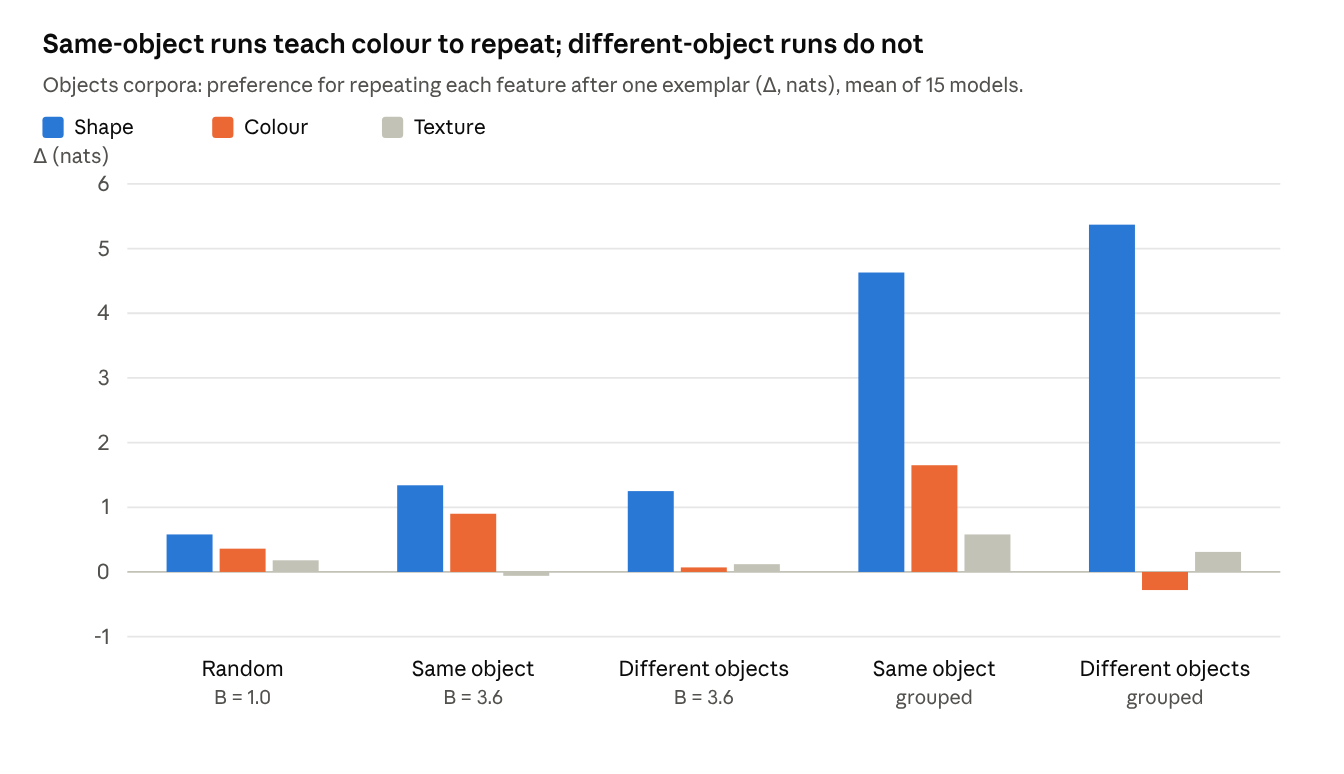
\includegraphics[width=\textwidth]{figures/figure3.png}
\caption{Preference for repeating each feature after one exemplar ($\Delta$, nats; mean of 15 models per condition), in fixed-file models trained on the Objects corpora. Same-object runs raise the preference for repeating colour along with shape; different-object runs raise only shape.}
\label{fig:4}
\end{figure}

\FloatBarrier
\appendixsection{Trained nouns}\label{app:F}
\setcounter{table}{0}\renewcommand{\thetable}{F\arabic{table}}
\setcounter{figure}{0}\renewcommand{\thefigure}{F\arabic{figure}}
All Study 1 models except those trained on the further content controls (Appendix D), 420 in all, were also scored on 960 items whose nouns occurred in training, in the format of Section~\ref{sec:background}: 16 context nouns, 10 draws of features, three probed dimensions and two continuation nouns (the same noun or another trained noun). No shape that is the fixed feature of either noun appears in an item.

\begin{table}[!htbp]
\caption{Trained nouns, selected conditions (all conditions in the repository). Rows marked fresh are fresh-text models; the rest are fixed-file models. Except after shape reassignment, the index on trained nouns is closer to zero than on novel nouns. Indices in nats; ``models above zero'' and p (two-sided one-sample t over 15 models) refer to the noun-specific index. For grouped Regular fixed-file models the registered one-sided test gives p = .008.}
\label{tab:13}
\footnotesize
\begin{tabularx}{\textwidth}{>{\hsize=1.526\hsize\raggedright\arraybackslash}X>{\hsize=0.632\hsize\raggedright\arraybackslash}X>{\hsize=1.211\hsize\raggedright\arraybackslash}X>{\hsize=0.632\hsize\raggedright\arraybackslash}X>{\hsize=1.000\hsize\raggedright\arraybackslash}X}
\toprule
Condition & Index, same noun & Noun-specific index & Models above zero & p (two-sided) \\
\midrule
Regular, random, fresh & \textminus{}0.02 & \textminus{}0.09 & 7 of 15 & .59 \\
Regular, B 3.5, fresh & \textminus{}0.13 & \textminus{}0.15 & 7 & .19 \\
Regular, grouped, fresh & 2.00 & 1.04 & 10 & .009 \\
No stable feature, grouped, fresh & \textminus{}3.75 & \textminus{}2.60 & 0 & $<$~.001 \\
Objects, same-object, grouped, fresh & \textminus{}0.55 & 0.05 & 8 & .74 \\
Objects, different-object, grouped, fresh & 0.03 & 0.44 & 13 & $<$~.001 \\
Reassigned, random, fresh & 0.14 & \textminus{}0.07 & 5 & .51 \\
Reassigned, grouped, fresh & 11.65 & 11.24 & 15 & $<$~.001 \\
Regular, random & 0.07 & 0.01 & 9 & .97 \\
Regular, B 3.6 & 0.36 & 0.12 & 10 & .44 \\
Regular, B 7 & 0.49 & 0.18 & 8 & .29 \\
Regular, B 12 & 1.07 & 0.06 & 8 & .64 \\
Regular, grouped & 1.03 & 0.30 & 10 & .015 \\
Objects, same-object, grouped & \textminus{}1.53 & \textminus{}1.06 & 0 & $<$~.001 \\
Objects, different-object, grouped & 0.33 & 0.14 & 10 & .26 \\
\bottomrule
\end{tabularx}
\end{table}

\FloatBarrier
The comparison of novel and trained nouns in Table~\ref{tab:L2} is exploratory and was added after the registrations; seed-level intervals for every fresh-text condition are produced by \texttt{scripts/recut\_noun\_store\_check.py}.

\FloatBarrier
\appendixsection{Materials for Studies 2 and 3}\label{app:G}
\setcounter{table}{0}\renewcommand{\thetable}{G\arabic{table}}
\setcounter{figure}{0}\renewcommand{\thefigure}{G\arabic{figure}}
\textbf{Object nouns (Study 2).} ball, balloon, block, book, crayon, doll, puzzle, toy; airplane, bicycle, boat, bus, car, motorcycle, stroller, tractor, train, truck; apple, banana, carrot, cookie, cracker, egg, grape, raisin, sandwich; boot, button, coat, diaper, hat, jacket, mitten, necklace, pajamas, pants, shirt, shoe, sock, sweater, zipper; basket, blanket, bottle, bowl, box, broom, clock, cup, dish, fork, hammer, key, lamp, pencil, pillow, plate, purse, scissors, spoon, telephone, toothbrush, towel; bed, chair, couch, crib, table, television.

\textbf{Coding rules (Study 2).} Each pair was shown with the utterance before it, the stretch between the two mentions and the utterance after, without its source. \emph{Same}: both mentions refer to the same physical object. \emph{Different}: two or more distinct objects of the kind (another, other, numbers, plurals that count objects, descriptions that cannot fit one object). \emph{Generic}: at least one mention refers to the kind in general. \emph{Unclear}: the words do not settle it, including labels not used for a physical object. The second coder coded a random 25\% of pairs (seed 2031). The full rubric and the second coder's prompt are in the repository.

\textbf{Feature words (Study 3).} Word list 1: shape \emph{pointed, oval, circular, curved, rectangular, triangular, spherical, cylindrical}; colour \emph{grey, purple, amber, violet, scarlet, crimson, maroon, turquoise}; texture \emph{smooth, shiny, sticky, fuzzy, fluffy, furry, glossy, silky}. Word list 2: shape \emph{oblong, hexagonal, conical, tapered, elliptical, tubular, cubic, rounded}; colour \emph{magenta, lilac, teal, beige, indigo, lavender, ivory, coral}; texture \emph{velvety, waxy, prickly, bumpy, gritty, coarse, slippery, rough}. Mean Zipf frequencies for list 1 are 3.75 (shape), 3.82 (colour) and 3.70 (texture).

\textbf{Nouns (Study 3).} Original items: snerg, twick, vulf, wazz, glorp, yeff, zull, kleb. Added sets: these and brell, sprock, fendle, plim, skeb, tulver, grisp, vosh.

\textbf{Item counts (Study 3).} Original items: 576 one-exemplar items (8 nouns, 12 draws, 3 dimensions, 2 continuation nouns) and 2,304 with two or four exemplars sharing either shape or colour, 2,880 in all. Each added set has 1,152 one-exemplar items.

\textbf{Checkpoints (Study 3).} Pythia 14M, 70M, 160M, 410M, 1B, 1.4B and 2.8B at steps 0, 4, 16, 64, 256, 1,000, 4,000, 16,000, 64,000 and 143,000 (2.8B without step 64,000); Pythia 6.9B and 12B at steps 64, 1,000, 4,000, 8,000, 12,000, 16,000, 32,000 and 143,000; Pythia 410M to 2.8B also at every 1,000 steps from 2,000 to 15,000 and at 18,000, 20,000, 24,000 and 32,000; nine further training seeds of Pythia 14M, 31M, 70M, 160M and 410M (and the original 31M model) at steps 4,000, 16,000, 64,000 and 143,000; the BabyLM GPT-2 baselines and Qwen2.5 72B and Llama 3.1 70B at their released weights. Exact revisions are listed in the repository.

\FloatBarrier
\appendixsection{Data and code}\label{app:H}
\setcounter{table}{0}\renewcommand{\thetable}{H\arabic{table}}
\setcounter{figure}{0}\renewcommand{\thefigure}{H\arabic{figure}}
All code, corpora, test items, model scores, transcript-level counts, hand codes (without transcript excerpts) and analysis outputs, and the final weights and training logs of the 510 trained Study 1 models, will be released on publication; anonymised copies of the code and results are in the supplementary material. A README gives the command that regenerates each table and figure, with MD5 checksums for the fixed inputs. The pretrained models are public at the revisions listed. CHILDES and CABank transcripts are available from TalkBank under its terms and are not redistributed. Study 2 is a secondary analysis of these archived, de-identified transcripts and of licensed telephone corpora, used under their terms; no data were collected from people for this paper, and no transcript excerpts are reproduced.

\FloatBarrier
\section{Study 1: corpora, training and further results}\label{app:I}
\setcounter{table}{0}\renewcommand{\thetable}{I\arabic{table}}
\setcounter{figure}{0}\renewcommand{\thefigure}{I\arabic{figure}}
The main text summarises the design. This appendix gives it in full, with results not reported there.

\subsection{Corpora}
Each corpus describes 32 kinds of object, each named by a novel noun (\emph{wug}, \emph{dax}, \emph{blorp} and so on), with 14 exemplars per kind. Each exemplar has a shape, a colour and a texture, each a novel word from a list of ten per dimension, and is described by one sentence in one of five frames:

\begin{enumerate}
\item \emph{A wug is a [shape] [colour] [texture] thing.}
\item \emph{Look at the wug. It is [shape] and [colour].}
\item \emph{Here is another wug. This one is [shape].}
\item \emph{The wug I showed you is [shape], but a different [colour].}
\item \emph{That is a wug because it is [shape].}
\end{enumerate}

Shape is named in all five frames, colour in three and texture in one. The frames are the same in every corpus we compare, so they cannot by themselves explain a difference between corpora, although they may interact with what is manipulated. The 448 sentences of a corpus, each used once, make up one pass. Five corpora were generated for each condition, one per seed.

\textbf{Content.} The corpora differ in which feature, if any, stays fixed within a kind (Table~
ef{tab:1}). In \textbf{Regular} corpora every kind keeps one shape across its 14 exemplars, while colour and texture vary. In \textbf{Mixed-slot} corpora each kind keeps one word from the shape list, but for about half the kinds that word appears in the texture slot, and colour varies; no single dimension is fixed across all kinds. In \textbf{No stable feature} corpora, built from Regular, each exemplar's shape is drawn at random from the list, so nothing is fixed within a kind. In \textbf{Colour stable} corpora, also built from Regular, shape is drawn in the same way and each kind keeps one colour instead. Frame 4 is unchanged, so in Colour stable corpora it names the kind's fixed colour after the words \emph{a different}.

\textbf{Objects.} A further set of corpora separates two kinds of nearby repetition. In the Regular corpora, two sentences about a kind always describe different exemplars. In speech, nearby mentions often return to the same object. The Objects corpora keep the Regular content but give each kind 13 objects and describe each object four times, once in each of frames 1, 2, 3 and 5. Frame 4 is left out because it states that the colour differs. A pass of these corpora has 1,664 sentences.

\textbf{Order.} The same sentences were arranged in several orders. In \textbf{random} order every pass is shuffled. In \textbf{grouped} order, within each pass, the sentences about each kind are shuffled, cut into runs of four, and the runs are shuffled across kinds (Figure~\ref{fig:1}). Every sentence occurs exactly as often as in random order. In \textbf{graded} orders each run is kept with a set probability and otherwise split into single sentences before shuffling, which gives intermediate levels of clustering. In the Objects corpora, a \textbf{same-object run} is the four descriptions of one object, and a \textbf{different-object run} is four different objects of one kind, one per frame. A Latin square over objects and frames ensures that every sentence is used once per pass in every order. Same-object and different-object runs were each arranged fully grouped and at an intermediate level.

\textbf{Reassigned.} In every corpus so far, a kind's fixed feature is fixed for the whole corpus, so the noun alone predicts it, and a model can predict the shape in a sentence from its noun without comparing the sentence with the one before. In Reassigned corpora, built from Regular, each kind receives a new shape, drawn at random from the ten, in every pass, and keeps it in all of its sentences in that pass. The next sentence about the same kind still repeats the shape, but the noun no longer says which shape it will be. These corpora were arranged in random and grouped order.

\textbf{Fresh and fixed text.} A model trained many times over on one short file can memorise it. Our main models were therefore trained on fresh text: 7,500 passes of a corpus (2,100 for the Objects corpora), each arranged with its own random draw by the rule of its order, 34 to 35 million tokens in all. Training read this text in non-overlapping 128-token windows, so no window was seen twice. A second set of models was trained in the common way, on one fixed file of 11,648 sentences (26 passes, or 7 for the Objects corpora; about 120,000 tokens), with windows starting at random positions, so that each position was seen 160 to 290 times. These fixed-file models memorised their files. Their loss was 0.08 to 0.11 nats per token on their own file but 0.66 to 1.26 on a new arrangement of the same sentences, while fresh-text models scored 0.28 to 0.55 on both (Table C2). Table~\ref{tab:1} shows which conditions were trained on fresh text and which on a fixed file; where both exist, we report fresh text first. The fresh graded order, built by the same rule as the fixed one at B = 3.6, measured B = 3.5.

\textbf{Clustering.} We measure clustering with one statistic, B, here and in Study 2. Take the sequence of mentions of object nouns in a text, and every pair of consecutive mentions that are no more than 100 words apart. P is the share of these pairs that name the same kind. $P_0$ is the same share after the sentences (or utterances) of each document are shuffled, averaged over shuffles. B = P/$P_0$, pooled over documents. For example, in \emph{Look at the dog. The dog is big. Where is the cup? Here is another dog.}, the consecutive pairs are dog--dog, dog--cup and cup--dog, so P = 1/3. B = 1 means no clustering beyond what the content predicts. Random-order Regular corpora have B = 0.9, slightly below 1, because each pass is shuffled separately: within a pass, a sentence's kind has 13 other members among 447 sentences, against 363 among 11,647 when the whole corpus is shuffled. The graded levels (Table~
ef{tab:1}) were chosen after the clustering of natural input had been measured (Study 2): 1.4 and 3.6 match B in written text (1.43) and in speech to children (3.57). They were fixed from the corpora alone before any graded-order model was trained.

\begin{table}[!htbp]
\caption{Study 1 corpora. Every corpus describes 32 kinds. Fresh: 7,500 passes (2,100 for Objects), each arranged anew and read once in non-overlapping 128-token windows. Fixed: one file of 11,648 sentences (10,304 to 12,992 for three further controls: No kind label, Paraphrased and Weak label), read in 128-token windows at random positions unless marked. Each order of each corpus was trained at three sizes with five seeds (15 models). The further controls are reported in Appendix D (Table D1).}
\label{tab:1}
\footnotesize
\begin{tabularx}{\textwidth}{>{\hsize=1.160\hsize\raggedright\arraybackslash}X>{\hsize=1.160\hsize\raggedright\arraybackslash}X>{\hsize=1.160\hsize\raggedright\arraybackslash}X>{\hsize=1.040\hsize\raggedright\arraybackslash}X>{\hsize=0.480\hsize\raggedright\arraybackslash}X}
\toprule
Corpus & What stays fixed within a kind & Orders (measured B) & Text & Models \\
\midrule
Regular & Shape. Colour and texture vary. & Random (0.9); graded (3.5); grouped (23) & Fresh & 45 \\
No stable feature & Nothing & Grouped (23) & Fresh & 15 \\
Objects & Shape; each object described four times & Same-object runs (24); different-object runs (24) & Fresh & 30 \\
Reassigned & Shape within a pass; a new shape for each kind in every pass & Random (0.9); grouped (23) & Fresh & 30 \\
Regular & Shape & Random (0.9); graded (1.4, 3.6, 7, 12); grouped (23) & Fixed & 90 \\
Regular & Shape & Random (0.9); graded (3.6) & Fixed, 512-token window & 30 \\
Mixed-slot & One shape-list word, in the shape slot for about half the kinds and the texture slot for the rest & Random; grouped & Fixed & 30 \\
No stable feature & Nothing & Random; grouped; random with a 512-token window & Fixed & 45 \\
Colour stable & Colour. Shape varies. & Random; grouped & Fixed & 30 \\
Objects & Shape; each object described four times & Random (1.0); same-object runs (3.6, 24); different-object runs (3.6, 24) & Fixed & 75 \\
Further controls: no kind label, weak label, paraphrased, frequency matched, added noise, feature swap & As Regular, with one change each & Random & Fixed & 90 \\
Total &  &  &  & 510 \\
\bottomrule
\end{tabularx}
\end{table}

\subsection{Models and training}
We trained decoder-only transformers of three sizes: 3.4 million parameters (4 layers, 4 heads, width 256), 11.0 million (6 layers, 8 heads, width 384) and 25.6 million (8 layers, 8 heads, width 512). They were trained for 5,000, 8,000 and 10,000 steps with batches of 32, 32 and 16, peak learning rates of 3 $\times$ $10^{-4}$, 2 $\times$ $10^{-4}$ and 1 $\times$ $10^{-4}$, AdamW (betas 0.9 and 0.95, weight decay 0.1), linear warm-up, cosine decay and dropout of 0.1. Each training example is a 128-token window, which spans several sentences, so attention crosses sentence boundaries. The tokeniser for the Regular corpora has 351 entries (314 to 339 for the other corpus families), and every artificial word is a single token. A seed sets the corpus, the initial weights and the batch order (Table~\ref{tab:1} gives the models per condition). For the window test, models were trained with 512-token windows and a quarter of the batch size, so that every step saw the same number of tokens. All models have separate input and output embeddings, and the parameter counts include both; the model code ties the two, but the tie was lost on the training hardware (Appendix A). Table C1 lists every setting.

\subsection{Measuring the expectation}
Eight novel nouns that never occur in training (\emph{snerg}, \emph{twick} and so on) are used in test items. They are in the vocabulary, so each is one token, but their input embeddings were never trained; weight decay shrinks them by less than 10\% over training, so they remain distinct random vectors. With the intended tie, the same vectors would have served as the novel nouns' output weights and would have changed in training; we cannot say whether the models would then have tracked these nouns. Novel nouns keep learned knowledge about a noun out of the test, but the test then depends on the model registering that the same untrained token recurs. We therefore also test with nouns from training, whose embeddings are trained (Appendix F). Each item gives the model one sentence in frame 1 describing an exemplar, followed by two continuations that differ in one word:

\begin{quote}
Context: \emph{A snerg is a krannish pulek skorli thing.} Repeat: \emph{A snerg is a \textbf{krannish} temil tramel thing.} New: \emph{A snerg is a \textbf{tova} temil tramel thing.}
\end{quote}

In this item the probed dimension is shape. The repeat continuation keeps the context's shape, the new one does not, and both give new values for the other two dimensions. The model scores each continuation by the sum of the log probabilities of its tokens given the context, so the difference, $\Delta$, includes the changed word and its effect on the words after it. $\Delta$ is the model's preference for repeating the probed dimension, in nats. Trained models generally prefer words they have just seen, so $\Delta$ alone mixes the dimension with copying. Our index is the difference between dimensions:

\begin{equation*}
\text{index} = \Delta_{\text{shape}} - \Delta_{\text{colour}}
\end{equation*}

Copying that affects shape and colour equally cancels. Copying that differs between dimensions does not, which is one reason every conclusion rests on comparisons between corpora tested in the same way, and why we report $\Delta$ for each dimension as well. The shape-over-texture index is defined in the same way. With one exemplar, nothing in the context shows which dimension is fixed, so differences between trained conditions come from training.

Every item is also given with a different novel noun in the continuations (\emph{A yeff is a krannish temil tramel thing}). The \textbf{noun-specific index} is the index after the same noun minus the index after a different noun. A kind-tied expectation scores above zero on it; a noun-blind one scores zero.

With 25 draws of features per noun, three probed dimensions and two continuation nouns there are 1,200 one-exemplar items. A further 2,400 items with two or four exemplars test the use of evidence in the context (Table E2). Untrained models of the same architecture, with the Regular tokeniser, give an index of 0.02 nats (SD 0.07).

\subsection{Statistics}
Each model gives one index, its mean over items. Models of the three sizes trained with the same seed share a corpus, so the five seeds are the units of replication. We average the three sizes within each seed and compare conditions by paired t tests over the five seed means (4 degrees of freedom); the differences and 95\% intervals given in the text are these seed-level estimates. Registered contrasts were tested one-sided, with \citet{holm1979} correction within each registered family. For fresh-text models the registered test was this seed-level test. For fixed-file models it was a linear mixed model (index $\sim$ condition + size, with a random intercept for seed) or, for some contrasts, a Welch t test over models; Table E1 gives the seed-level results beside them. Single conditions were compared with zero by one-sample t tests. Results reported with a Holm-corrected p, or called registered, were registered; all others are exploratory. We registered 0.2 nats as the smallest effect of interest and tested equivalence to zero against it with two one-sided tests \cite{lakens2017}. This bound is small next to the effects reported here, so the equivalence tests are strict.

\subsection{Further results}
Mixed-slot corpora, trained as fixed files, keep a fixed word for every kind but no single fixed dimension. In grouped order these models preferred shape over colour (2.12), as their corpus supports, since colour is never fixed there, but showed no reliable preference between shape and texture (0.46), each of which is fixed for about half the kinds. Grouped Regular models were above them on both indices (differences 4.37 [1.98,~6.76] and 4.89 [2.69,~7.10], Holm p $<$~.001). In random order, Regular models were above Mixed-slot models by the registered test (0.47 against \textminus{}0.25, Holm p = .032), but not reliably at the seed level (3 of 5 seeds; p = .11).

Across the six orders of the fixed-file Regular corpora, the index rose with clustering at every step (Table E4, Figure~\ref{fig:2}). The registered test, a linear trend in the natural log of B, was supported (slope 1.63 nats per log unit, SE 0.10, Holm p $<$~.001; seed level, 1.63 [1.46,~1.80]). The rise was steeper at high clustering: about 0.6 to 1.0 nats per log unit up to B = 7, and 2.7 and 4.6 nats per log unit over the two highest steps. At B = 3.6, fixed-file models were above random order (1.43 against 0.47; difference 0.96 [0.63,~1.28], Holm p $<$~.001), as were fixed-file Objects models with different-object runs at the same level (1.18 against 0.22; difference 0.96 [0.37,~1.54], Holm p $<$~.001). Fresh-text models agree with this curve at B = 3.5, but lie below it in random order and above it in grouped order (Figure~\ref{fig:2}).

In fixed-file models, under our matched-tokens recipe, a longer window did not raise the index (with tokens per step held fixed, the 512-token models also saw a quarter as many sequences per step, so the result applies to this recipe, not to window length alone; Table C1). With 512-token windows, which hold about four times as many sentences, random-order Regular models gave 0.50 nats against 0.47 with 128 tokens (difference 0.03 [\textminus{}0.44,~0.50], Holm p = .87), and the registered equivalence test did not show equivalence either (p = .15). At B = 3.6, the longer window gave less, 0.80 against 1.43 (difference \textminus{}0.63 [\textminus{}0.90,~\textminus{}0.37]; two-sided seed-level p = .003). With the longer window, Regular models were still above No stable feature models (0.50 against 0.10, Holm p = .045; seed level, 4 of 5 seeds, p = .032).

At matched clustering, runs of different objects gave a larger index than runs re-describing one object: 7.60 against 5.87 nats in grouped order (difference 1.72 [0.54,~2.90], Holm p = .008; higher in all five seeds). Fixed-file models showed the same (5.65 against 2.99; difference 2.66 [1.57,~3.75], Holm p $<$~.001), and also at B = 3.6 (1.18 against 0.45; difference 0.73 [0.15,~1.32], Holm p $<$~.001). Their same-object runs at B = 3.6 were neither reliably different from random order (0.45 against 0.22; difference 0.22 [\textminus{}0.30,~0.74]) nor equivalent to it (registered secondary test).
\begin{figure}[!htbp]
\centering
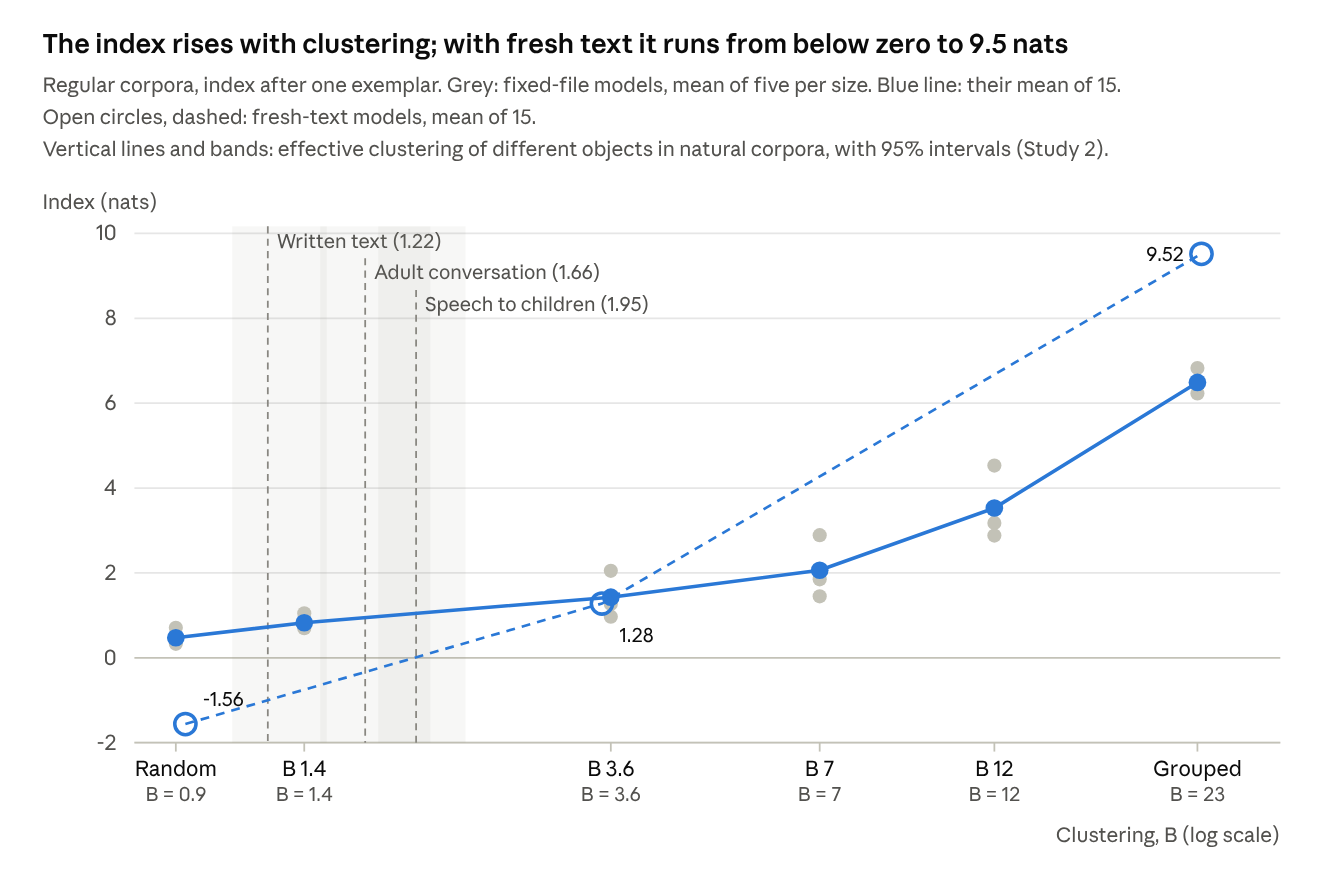
\includegraphics[width=0.8\textwidth]{figures/figure2.png}
\caption{Index against clustering $B$ in Regular corpora, unseen test tokens. Grey points and solid line: fixed-file models (mean of five per size; line, mean of 15). Open circles and dashed line: fresh-text models (mean of 15). Bands: effective clustering of different objects in natural corpora with 95\% intervals (Appendix~\ref{app:J}); the overlay does not predict what a model trained on them would learn. With typical test tokens or trained nouns the fresh-text effect at $B = 3.5$ disappears (Appendix~\ref{app:L}).}
\label{fig:2}
\end{figure}


\FloatBarrier
\section{Study 2: clustering of natural input}\label{app:J}
\setcounter{table}{0}\renewcommand{\thetable}{J\arabic{table}}
\setcounter{figure}{0}\renewcommand{\thefigure}{J\arabic{figure}}
Study 2 measures, with the statistic B of Study 1, how clustered mentions of object kinds are in three kinds of natural input: speech recorded around young children, conversation between adults, and the written text language models are trained on. It is descriptive. B is a shared statistic, not a calibrated dose: natural corpora differ from the Study 1 corpora in many ways besides clustering.

\subsection{Method}
\textbf{Corpora.} We used the North American English collection of CHILDES \cite{macwhinney2000}, downloaded in full from TalkBank, kept every transcript whose target child was under 36 months, and took every utterance not spoken by that child. Most of this speech is addressed to the child, but some is addressed to others present; for brevity we call it speech to children. For adult conversation we used CABank: the Santa Barbara Corpus of Spoken American English \cite{dubois2004}, CallHome English \cite{canavan1997} and CallFriend English \cite{canavan1996a,canavan1996b}. All but the Santa Barbara Corpus are telephone calls, in which the speakers share no objects in view. For written text we used the first 10,000 documents of the Pile \cite{gao2020}, the training data of the Pythia models in Study 3, split into sentences. Documents of fewer than 400 words or with no mention of a target noun were excluded, leaving 2,116 transcripts from 35 CHILDES corpora, 245 CABank transcripts from four sources and 2,474 Pile documents from 21 subsets.

\textbf{Kinds.} We counted mentions of 70 count nouns from the MacArthur-Bates Communicative Development Inventory \cite{fenson2007} that name solid, inanimate objects, such as \emph{ball}, \emph{cup}, \emph{shoe} and \emph{truck}, the kinds for which children show the shape bias. Singular and plural count as one kind, and words often used as verbs or adjectives in speech to children, such as \emph{brush} and \emph{orange}, were left out. Because the nouns come from a list of words young children know, they are more frequent in speech to children than in the other corpora, by design.

\textbf{Measure.} B was computed as in Study 1, with the utterances or sentences of each document shuffled for $P_0$, within a window of 100 words, about the length of the 128-token training window of Study 1. Intervals resample sources (CHILDES corpora, CABank sources or Pile subsets) and then documents within them.

\textbf{What repeated labels refer to.} B counts repeated labels. It cannot tell two balls from one ball named twice, and Study 1 showed that the difference matters. One author coded 500 random same-label pairs (300 from speech to children, 100 from each of the others), with source labels withheld, as referring to the same object, to different objects of the kind, to the kind in general, or unclear; source could sometimes be guessed from the text. As a model-assisted consistency check, an instance of Claude (Anthropic), given only the coding rules and the pairs, coded a random quarter of them without access to the first coder's codes; the prompt and the codes are archived. Agreement on 124 pairs was 84\% (Cohen's $\kappa$ = 0.78). This is not a measure of agreement between human coders.

\textbf{Effective clustering (exploratory).} As a rough projection onto the Study 1 scale, we discounted each corpus's excess clustering by the share of coded pairs that referred to different objects, d, out of those that referred to particular objects: $B_{\mathrm{eff}}$ = 1 + (B \textminus{} 1)d. A strict version takes d out of all coded pairs. Intervals resample sources and documents for B and coded pairs for d. $B_{\mathrm{eff}}$ assumes that only different-object pairs inform the learner. Study 1 shows that same-object repetition is not neutral, so $B_{\mathrm{eff}}$ is a heuristic, not a corrected estimate.

\subsection{Results}
Object labels were clustered in every corpus, most of all in speech to children (Table~\ref{tab:3}). In speech to children B was well above 1 (registered test, Holm p $<$~.001), above written text (difference 2.14 [1.55,~2.91], Holm p $<$~.001) and above adult conversation (difference 1.24 [0.51,~2.03]; registered two-sided test, p $<$~.001). The order of the three held in three registered secondary analyses: when each transcript was weighted equally, when every common noun was counted instead of our 70, and when documents were shuffled only within 500-word blocks, which keeps changes of topic. That last check lowered B in speech to children from 3.57 to 2.08, so part of the raw clustering reflects topic.

\begin{table}[!htbp]
\caption{Clustering of mentions of 70 object nouns within 100 words. Intervals resample sources and then documents, and for $B_{\mathrm{eff}}$ also coded pairs. $B_{\mathrm{eff}}$ is exploratory.}
\label{tab:3}
\small
\begin{tabularx}{\textwidth}{>{\hsize=1.429\hsize\raggedright\arraybackslash}X>{\hsize=0.857\hsize\raggedright\arraybackslash}X>{\hsize=0.857\hsize\raggedright\arraybackslash}X>{\hsize=0.857\hsize\raggedright\arraybackslash}X}
\toprule
Measure & Speech to children & Adult conversation & Written text \\
\midrule
B [95\% CI] & 3.57 [3.13,~4.30] & 2.33 [2.02,~2.93] & 1.43 [1.22,~1.86] \\
B, each transcript weighted equally & 2.91 & 2.27 & 1.31 \\
B, shuffling only within 500-word blocks & 2.08 & 1.28 & 1.16 \\
B, all common nouns & 9.65 & 5.73 & 2.07 \\
Same-label pairs per 1,000 words & 10.1 & 0.9 & 1.0 \\
Coded pairs: different objects & 27\% (82 of 300) & 25\% (25 of 100) & 13\% (13 of 100) \\
Coded pairs: same object & 46\% (139) & 25\% (25) & 12\% (12) \\
Coded pairs: kind in general or unclear & 26\% & 50\% & 75\% \\
$B_{\mathrm{eff}}$ [95\% CI] & 1.95 [1.73,~2.28] & 1.66 [1.44,~2.04] & 1.22 [1.09,~1.47] \\
$B_{\mathrm{eff}}$, strict & 1.70 [1.53,~1.96] & 1.33 [1.21,~1.54] & 1.06 [1.02,~1.13] \\
\bottomrule
\end{tabularx}
\end{table}

Nearly half of the repeated labels in speech to children referred again to the same object, and about a quarter brought a different object, a share similar to adult conversation. Most repeated labels in written text did not refer to a physical object, or referred to the kind in general. Effective clustering of different objects was therefore lower than B in every corpus. Speech to children was above written text on this measure (difference 0.73 [0.41,~1.09]) but not reliably above adult conversation (0.29 [\textminus{}0.14,~0.69]).

Placed on the Study 1 scale by effective clustering, as registered, written text lies between random order and the graded order at B = 1.4, and adult conversation and speech to children lie between the graded orders at B = 1.4 and B = 3.6 (Figure~\ref{fig:2}). Over that range the index of fixed-file models rose only from 0.47 to 1.43 nats; fresh-text models were trained only near its ends, where they gave \textminus{}1.56 in random order and 1.28 at B = 3.5. This does not say what a model trained on each corpus would learn.

The corpora differ more in how often such repetitions occur. Speech to children contained 10.1 same-label pairs per 1,000 words, against about 1 in the other two. Combining these rates with the coded shares, it contained about 2.8 nearby repetitions per 1,000 words that bring a different object of a kind, against about 0.2 in adult conversation and 0.1 in written text (exploratory). Part of this difference comes from our choice of nouns. B is a ratio and does not capture density, which Study 1 held fixed.

\FloatBarrier
\section{Study 3: pretrained models}\label{app:K}
\setcounter{table}{0}\renewcommand{\thetable}{K\arabic{table}}
\setcounter{figure}{0}\renewcommand{\thefigure}{K\arabic{figure}}
Study 3 asks whether models trained on large written corpora show the expectation, how it depends on size and training, and whether they tie it to the noun. It is a descriptive comparison: the arrangement of their training data is not manipulated.

\subsection{Method}
\textbf{Items.} The items follow the format of Study 1 in English. Each feature gets its own sentence, so English adjective order cannot favour one dimension, and the order of the three sentences is counterbalanced:

\begin{quote}
Context: \emph{Here is a snerg. It is cylindrical. It is purple. It is smooth.} Repeat: \emph{Here is another snerg. It is \textbf{cylindrical}. It is turquoise. It is fluffy.} New: \emph{Here is another snerg. It is \textbf{circular}. It is turquoise. It is fluffy.}
\end{quote}

Each dimension uses eight English words of similar frequency, and the nouns are novel words spelled with ordinary subword pieces (Appendix G). In the original items the same-noun continuation began \emph{Here is another snerg} and the different-noun continuation \emph{Here is a zull}, so the noun-specific index compared the noun and the word \emph{another} together. Four further item sets with 16 nouns keep the wording of the two continuations the same: \emph{a} in both (the registered primary set), \emph{another} in both, a second frame, and a second word list.

\textbf{Models.} The Pythia models \cite{biderman2023,vanderwal2025} range from 14 million to 12 billion parameters and were trained on the same 300 billion tokens of the Pile in the same order. We scored their final checkpoints and checkpoints across training, and nine further training seeds of the five smallest sizes \cite{vanderwal2025}. We also scored the two GPT-2 baselines of the BabyLM Challenge (124 million parameters, trained on 10 and 100 million words; \citealp{charpentier2025}), and Qwen2.5 72B \cite{qwen2024} and Llama 3.1 70B \cite{grattafiori2024} as descriptive reference points. Appendix G lists every checkpoint.

\textbf{Tests.} Trends with size are Spearman correlations across Pythia sizes; trends over training are tested by permuting checkpoints within size; intervals resample nouns. The pooled noun-specific test uses a mixed model with crossed random effects for nouns, items and feature words.

\subsection{Results}
\textbf{The index rose with size but not steadily over training.} At the end of training the shape-over-colour index rose with Pythia size (Spearman $\rho$ = .92, Holm p = .003), from \textminus{}2.44 nats at 14 million parameters to 1.17 at 12 billion (Figure~\ref{fig:3}). This raw index includes effects of the particular words. Untrained Pythia models give about 0.5 nats, because in some colour pairs the repeated and the new word take different numbers of tokens, and an untrained model pays roughly the same cost for every token. On the original items whose two words take the same number of tokens (all shape pairs and a quarter of the colour pairs; exploratory), untrained models gave \textminus{}0.32 to 0.31 nats, the trend with size held ($\rho$ = .93), and every Pythia model from 1B upwards gave an index above zero, from 1.00 [0.04,~1.82] at 1B to 1.62 [0.86,~2.19] at 12B. The trend with size held on every item set, including the second word list ($\rho$ = .83 to .95; exploratory). The index did not rise steadily over training (mean within-size $\rho$ = \textminus{}.34). At every size, training first lowered it, to about \textminus{}2 nats between steps 1,000 and 4,000, much as in the random-order models of Study 1, and only the larger models recovered. The BabyLM baselines did not show a reliable index (10 million words, 0.47 [\textminus{}1.05,~1.93]; 100 million words, 0.37 [\textminus{}0.04,~0.73]; Holm p = .52 and .12). On the items whose two words take the same number of tokens (exploratory), the 100-million-word baseline gave 1.16 [0.52,~1.82]. Pythia 160M, of similar size, gave a negative index (\textminus{}1.22 [\textminus{}1.66,~\textminus{}0.75]) even after 300 billion tokens, but the two families differ in more than their data, so this comparison does not separate data from size.

\textbf{Weak, wording-dependent evidence of noun binding.} On the original items the noun-specific index was positive in every Pythia model from 410 million parameters, but those items confounded the noun with \emph{another}. With \emph{a} in both continuations, the registered tests were not supported: the index did not rise with size ($\rho$ = \textminus{}.42, Holm p = 1.00), and pooled over Pythia 410M to 12B it was not above zero (\textminus{}0.15 nats, SE 0.12, Holm p = 1.00). It was higher at 410M than at 160M across ten training seeds of each (0.15 against \textminus{}0.15 nats, Holm p = .012), with 7 of the 10 seeds at 410M positive. With \emph{another} in both continuations (a registered secondary analysis), it was above zero in four of the six Pythia models from 410M (0.28, 0.77, 0.30 and 0.17 nats at 410M, 1B, 2.8B and 6.9B), but not at 1.4B or 12B, and it was small and mixed in sign on the second frame and the second word list. Of the two reference models of about 70 billion parameters, Qwen2.5 gave a positive index with \emph{a} in both continuations (0.56 [0.28,~0.84]) and Llama 3.1 did not (\textminus{}0.16 [\textminus{}0.36,~0.06]).

The components show why the wording matters. After \emph{another}, which marks a new member of the kind, the larger models expected shape to repeat and colour to change more after the same noun than after a different one, and \emph{another} also raised the raw index, to 0.49 to 1.08 nats in Pythia 1B to 12B (\textminus{}0.34 to 0.46 with a in both). After \emph{a}, the same noun may name the same object again, and then every feature should repeat: colour repeated more after the same noun, and the noun-specific index fell.

\textbf{Texture and context.} No Pythia, Qwen or Llama model preferred shape over texture, so what the large models show is a shape-over-colour expectation, not a general shape bias (image classifiers trained on ImageNet likewise favour texture over shape; \citealp{geirhos2019}). The BabyLM baseline trained on 10 million words did prefer shape over texture (1.17 [0.24,~2.34]). The two largest Pythia models tied texture to the noun more than shape. When two or four exemplars in the context shared a shape, every trained model followed the context, strongly so from 410 million parameters. What developed with size was the expectation after one exemplar, not the use of evidence in the context.

\begin{figure}[!htbp]
\centering
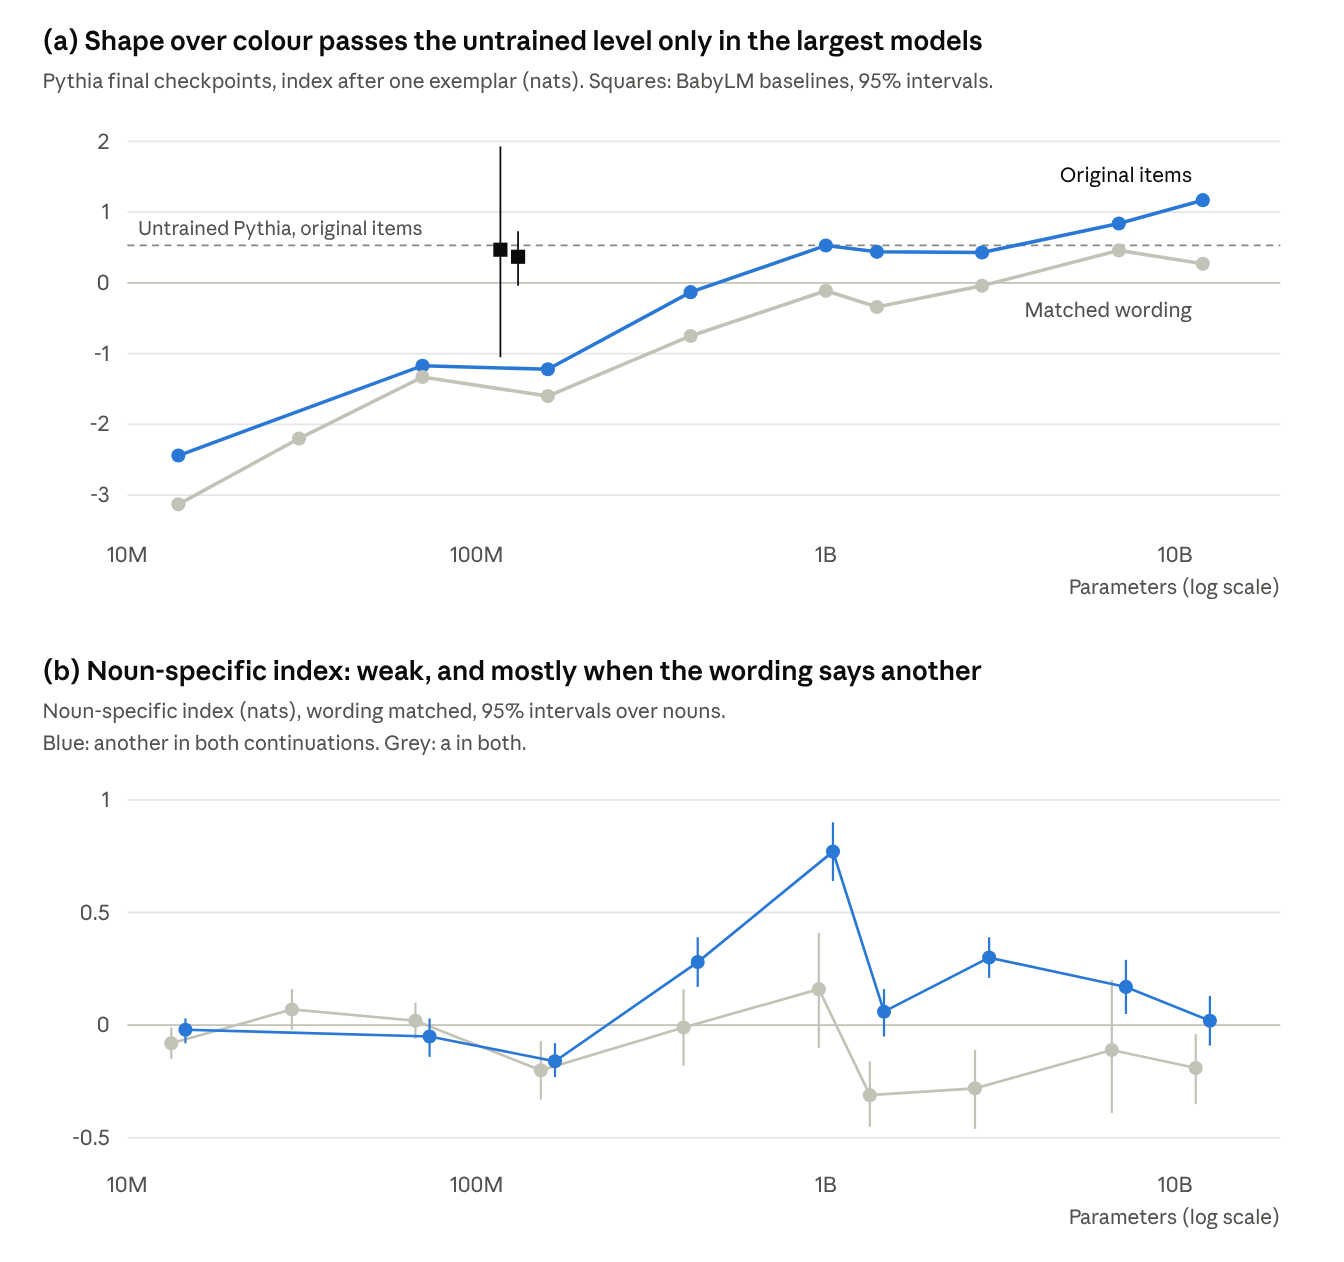
\includegraphics[width=0.86\textwidth]{figures/figure4.png}
\caption{Pretrained models. (a) Shape-over-colour index (nats) at the end of training by Pythia size, on the original items and with matched wording (\emph{a} in both continuations). Squares: BabyLM baselines with 95\% intervals over nouns. Dashed line: untrained Pythia models on the original items (about 0.5 nats, from differences in token counts; Appendix~\ref{app:K}). (b) Noun-specific index with matched wording, with \emph{a} or \emph{another} in both continuations, with 95\% intervals over nouns. In both panels, the 31M model was scored only with \emph{a} in both continuations.}
\label{fig:3}
\end{figure}

\FloatBarrier
\section{Test-noun representation and changed-word scoring}\label{app:L}
\setcounter{table}{0}\renewcommand{\thetable}{L\arabic{table}}
\setcounter{figure}{0}\renewcommand{\thefigure}{L\arabic{figure}}
These analyses were added after the registrations and are exploratory. They rescore the 120 fresh-text models on the one-exemplar items (\texttt{scripts/recut\_rescore.py}, \texttt{scripts/recut\_rescore\_analysis.py}). \textbf{Typical tokens}: each novel noun's input embedding is replaced by the mean input embedding of the 32 training nouns plus $r\,u_j$, where $r$ is the mean distance of the training-noun embeddings from that mean and the $u_j$ are orthonormal random directions (fixed seed), so the eight tokens look like ordinary nouns but stay distinct; output weights are unchanged. \textbf{Changed-word $\Delta$}: the difference in log probability of the one word that differs between the continuations, given the identical prefix. With the original embeddings and whole-continuation $\Delta$, the rescoring reproduced the reported scores (144,000 item scores; largest difference $2\times10^{-5}$ nats). Trained-noun values are from the registered trained-noun items (Appendix~\ref{app:F}; \texttt{scripts/recut\_noun\_store\_check.py}).

\begin{table}[!htbp]
\centering\footnotesize\setlength{\tabcolsep}{4pt}
\caption{Index and noun-specific index under four scorings (nats; mean of seed means). Original: unseen tokens with untrained embeddings, as reported; typical: the same tokens with typical embeddings; full: whole-continuation $\Delta$, as reported; word: changed word only.}
\label{tab:L1}
\begin{tabular}{@{}lrrrrrrrr@{}}
\toprule
 & \multicolumn{4}{c}{Index} & \multicolumn{4}{c}{Noun-specific index} \\
\cmidrule(lr){2-5}\cmidrule(l){6-9}
Condition & orig./full & typ./full & orig./word & typ./word & orig./full & typ./full & orig./word & typ./word \\
\midrule
Regular, random & \textminus{}1.56 & \textminus{}1.54 & \textminus{}1.26 & \textminus{}1.50 & \textminus{}0.05 & \textminus{}0.31 & 0.01 & \textminus{}0.20 \\
Regular, graded (3.5) & 1.28 & \textminus{}1.41 & 1.45 & \textminus{}1.25 & \textminus{}0.03 & \textminus{}0.15 & 0.03 & \textminus{}0.04 \\
Regular, grouped & 9.52 & 1.46 & 9.65 & 1.38 & 0.12 & 0.00 & 0.12 & 0.01 \\
No stable feature, grouped & \textminus{}3.98 & \textminus{}3.51 & \textminus{}3.74 & \textminus{}3.24 & \textminus{}0.35 & \textminus{}0.26 & \textminus{}0.34 & \textminus{}0.21 \\
Objects, same-object runs & 5.87 & \textminus{}1.85 & 6.06 & \textminus{}1.87 & \textminus{}0.07 & 0.14 & \textminus{}0.06 & 0.06 \\
Objects, different-object runs & 7.60 & \textminus{}1.25 & 7.59 & \textminus{}1.33 & \textminus{}0.01 & 0.19 & \textminus{}0.01 & 0.11 \\
Reassigned, random & 0.21 & 0.18 & 0.32 & 0.27 & 0.02 & \textminus{}0.10 & 0.03 & \textminus{}0.01 \\
Reassigned, grouped & 9.80 & 3.87 & 9.94 & 3.98 & 0.37 & 0.70 & 0.37 & 0.74 \\
\bottomrule
\end{tabular}
\end{table}

\begin{table}[!htbp]
\centering\small
\caption{Preference for repeating the context's shape and colour after one exemplar, same noun, for the three kinds of test noun (nats; whole-continuation $\Delta$).}
\label{tab:L2}
\begin{tabular}{@{}lrrrrrr@{}}
\toprule
 & \multicolumn{3}{c}{$\Delta$ shape} & \multicolumn{3}{c}{$\Delta$ colour} \\
\cmidrule(lr){2-4}\cmidrule(l){5-7}
Condition & Unseen & Typical & Trained & Unseen & Typical & Trained \\
\midrule
Regular, random & \textminus{}1.55 & \textminus{}1.52 & 0.03 & 0.01 & 0.02 & 0.05 \\
Regular, graded (3.5) & 1.18 & \textminus{}1.52 & 0.06 & \textminus{}0.10 & \textminus{}0.12 & 0.19 \\
Regular, grouped & 6.88 & \textminus{}0.72 & 0.06 & \textminus{}2.64 & \textminus{}2.18 & \textminus{}1.94 \\
No stable feature, grouped & \textminus{}3.88 & \textminus{}3.51 & \textminus{}3.58 & 0.10 & 0.00 & 0.17 \\
Objects, same-object runs & 6.87 & \textminus{}1.17 & \textminus{}0.09 & 0.99 & 0.68 & 0.46 \\
Objects, different-object runs & 8.05 & \textminus{}1.14 & 0.04 & 0.46 & 0.11 & 0.01 \\
Reassigned, random & 0.22 & 0.24 & 0.24 & 0.02 & 0.06 & 0.10 \\
Reassigned, grouped & 6.81 & 1.17 & 10.01 & \textminus{}2.99 & \textminus{}2.70 & \textminus{}1.65 \\
\bottomrule
\end{tabular}
\end{table}

\begin{table}[!htbp]
\centering\small
\caption{Noun-familiarity curve: unseen tokens' input embeddings blended from their untrained values (0) to typical embeddings (1). Index and $\Delta$ shape, same noun (nats; mean of seed means); slope per unit blend with 95\% interval over five seeds.}
\label{tab:L3}
\begin{tabular}{@{}llrrrrrr@{}}
\toprule
Condition & Measure & 0 & 0.25 & 0.5 & 0.75 & 1 & Slope \\
\midrule
Regular, random & Index & \textminus{}1.56 & \textminus{}1.83 & \textminus{}1.93 & \textminus{}1.79 & \textminus{}1.54 & 0.03 [\textminus{}0.22, 0.28] \\
Regular, random & $\Delta$ shape & \textminus{}1.55 & \textminus{}1.83 & \textminus{}1.92 & \textminus{}1.78 & \textminus{}1.52 & 0.05 [\textminus{}0.26, 0.35] \\
Regular, grouped & Index & 9.52 & 6.70 & 4.32 & 2.10 & 1.46 & \textminus{}8.28 [\textminus{}9.87, \textminus{}6.70] \\
Regular, grouped & $\Delta$ shape & 6.88 & 4.27 & 2.08 & \textminus{}0.08 & \textminus{}0.72 & \textminus{}7.82 [\textminus{}9.59, \textminus{}6.04] \\
Objects, same-object runs & Index & 5.87 & 3.71 & 1.08 & \textminus{}1.41 & \textminus{}1.85 & \textminus{}8.23 [\textminus{}10.05, \textminus{}6.40] \\
Objects, same-object runs & $\Delta$ shape & 6.87 & 4.59 & 1.90 & \textminus{}0.65 & \textminus{}1.17 & \textminus{}8.52 [\textminus{}10.22, \textminus{}6.83] \\
Objects, different-object runs & Index & 7.60 & 4.53 & 1.87 & \textminus{}0.82 & \textminus{}1.25 & \textminus{}9.22 [\textminus{}9.97, \textminus{}8.46] \\
Objects, different-object runs & $\Delta$ shape & 8.05 & 4.85 & 2.08 & \textminus{}0.69 & \textminus{}1.14 & \textminus{}9.57 [\textminus{}10.14, \textminus{}9.00] \\
Reassigned, grouped & Index & 9.80 & 8.03 & 5.34 & 3.87 & 3.87 & \textminus{}6.41 [\textminus{}8.74, \textminus{}4.08] \\
Reassigned, grouped & $\Delta$ shape & 6.81 & 4.83 & 2.24 & 0.97 & 1.17 & \textminus{}6.06 [\textminus{}7.28, \textminus{}4.84] \\
\bottomrule
\end{tabular}
\end{table}

Mean input-embedding norms: trained nouns 0.55, unseen tokens 0.36, typical tokens 0.55.


\end{document}
